% ===================================================================
% Arquivo: capitulos/parte-III-pilares/cap-08-retificadoras.tex
% ===================================================================

\chapter{Funções de Ativação Retificadoras}
\label{cap:ativacao-retificadoras}

\begin{flushright}
\textit{"caramba! A perda do meu modelo está em 31.415"} \\
--- Estagiário conhecendo o problema dos gradientes explosivos
\end{flushright}

% ===================================================================
% Resumo do capítulo
% ===================================================================

\section{Exemplo Ilustrativo: Vendendo Pipoca}

Imagine que você está querendo ganhar dinheiro e decidiu vender pipoca em uma praça da sua cidade. Você comprou milho, óleo, sal e manteiga, um carrinho para poder levar e fazer as pipocas, além disso, você também comprou vários pacotes para poder colocar as pipocas para vender.

Nisso, você teve que estipular um valor para vender essas pipocas, após pensar um pouco e analisar todos os seus gastos, você estimou que um valor de R\$ 5,00 seria ideal, pois conseguiria pagar os seus gastos mas você ainda ia obter lucro dos seus clientes.

Agora você está pronto para vender, começou a fritar o milho e colocou uma plaquinha com o preço ao lado do seu carrinho. Então chega uma pessoa com R\$ 6,00 e decide comprar um pacote, você vende e entrega um real de troco. Logo em seguida aparece uma segunda pessoa com R\$ 4,99 e decide negociar com você, ela afirma que é quase R\$ 5,00, e por isso, você deveria vender a pipoca para ela, mas você explica que só vende pelo valor de R\$ 5,00.

Com base nisso, nós podemos chegar em uma situação em que um pacote de pipoca será vendido somente se uma pessoa possuir R\$ 5,00 no bolso, ou mais. Podemos então escrever algo como o da equação \ref{eq: VendaPipoca}. Em casos em que uma venda ocorre, você poderá vender mais um pacote, para isso, o seu comprador deverá possuir pelo menos R\$ 10,00, assim, $x$ que indica a quantidade de pacotes vendido seguirá a lei de formação $x = 5 \mod d$, em que $d$ é o dinheiro que a pessoa possui.

\begin{equation}
    \text{Número de Pacotes} = \begin{cases} 0 & \text{quando } R\$ \leq  4,99 \\ x & \text{quando } R\$ > 4,99 \end{cases}
    \label{eq: VendaPipoca}
\end{equation}

Saindo do assunto da pipoca e voltando para o tema deste texto, existe uma família de funções de ativação que funciona de forma semelhante a lógica de venda dos pacotes de pipoca, elas são as unidades lineares retificadoras. A ReLU, que dá nome a essa família, funciona de forma semelhante a essa venda, ela tem um comportamento de "tudo ou nada", em que irá comandar quando um neurônio de uma rede neural irá disparar seu resultado.

As funções retificadoras, como a ReLU, são o tópico principal deste texto, para isso, antes de conhecê-las vamos entender um pouco do cenário que elas surgiram, com uso das funções sigmoides e o problema do gradiente em fuga. Em seguida veremos a ReLU os problemas que ela pode causar em uma rede neural. Seguindo adiante, conheceremos as suas variantes com vazamento, como a Leaky ReLU, depois as variantes suaves, como a ELU. Para conhecermos todas essas funções, serão utilizados gráficos, equações, comparativos de pesquisas e citações que explicam sobre suas propriedades. No final, veremos um comparativo com essas funções utilizando a construção de uma rede neural convolucional com o dataset CIFAR-10.

% ===================================================================
% ReLU
% ===================================================================

\section{Rectified Linear Unit (ReLU): A Revolução Retificadora}

Como foi visto anteriormente no capítulo \ref{cap:ativacao-sigmoidais}, as funções sigmoidais surgiram com inspiração nos neurônios humanos e como eles se comportam com determinados estímulos. Mas essas não foram as únicas funções que tiveram essa origem. Na década de 40, o pesquisador Alton Householder estava estudando um cenário parecido em seu trabalho \textit{A theory of steady-state activity in nerve fiber network: I. Definition of mathematical biofysics}, nele o autor analisou o comportamento de fibras nervosas e quando elas irão assumir caráter excitatório ou inibitório, para isso ele apresentou a equação \ref{eq:fibra-nervosa-householder} \parencite{Householder1941}.

\begin{equation}
    a_{ij} = \begin{cases} 0 & \text{quando } \eta_i \le h_{ij} \\ a_{ij}, & \text{quando } \eta_i > h_{ij} \end{cases}
    \label{eq:fibra-nervosa-householder}
\end{equation}

Essa equação nos mostra quando uma fibra nervosa irá disparar, para isso, devemos olhar o limiar da fibra $h_{ij}$ e o estímulo total $\eta_i$, com base nesses valores e no que a fórmula apresenta, uma fibra irá disparar quando o estímulo total for maior que o seu limiar, quando isso não ocorrer, ela não irá disparar \parencite{Householder1941}. Além disso, \textcite{Householder1941} explica também sobre o termo $a_{ij}$, a saída dessa função, segundo o autor ele é utilizado para representar o parâmetro de atividade, sendo um valor diferente de zero, podendo ser positivo (quando a fibra possui ação excitatória), ou negativo (apresentando caráter inibitório).

Essa equação criada por Householder, nos lembra bastante a expressão da função ReLU, a qual é denotada pelas fórmulas \ref{eq:relu}.

\begin{equacaodestaque}{Rectified Linear Unit (ReLU)}
    \text{ReLU}(z_i) = \begin{cases}z_i, & \text{se } z_i > 0 \\0, & \text{se } z_i \leq 0\end{cases} \text{ou} \text{ReLU}(z_i) = \max(0, z_i)
    \label{eq:relu}
\end{equacaodestaque}

Dito isso, mesmo com ela existindo a mais de 80 anos, ela só passou a ser amplamente utilizada nos anos 2010, antes disso, as sigmoides eram a grande maioria quando o assunto era função de ativação. Contudo, as sigmoides eram funções saturantes, e isso fazia com que sua derivada retornasse muitos valores pequenos ao longo da função. Ao multiplicar vários valores pequenos na retropropagação do gradiente, o vetor gradiente ia diminuindo até chegar um ponto em que ele não conseguia atualizar os pesos e vieses das redes neurais de forma eficiente, assim, tínhamos o problema do gradiente em fuga. As funções retificadoras, sendo a principal delas a ReLU, surgem para corrigir esse problema crônico. 

Dessa forma antes de conhecermos de fato a ReLU e suas propriedades, vamos antes entender o cenário que ela se popularizou, com os cientistas buscando novos tipos de funções de ativação que substituísse as sigmoides, funções saturantes, por outro tipo de função que resolvesse o problema do gradiente em fuga.

Nesse cenário, artigos como \textit{Rectified Linear Units Improve Restricted Boltzmann Machines} foram essenciais para popularizar a ReLU como uma função de ativação interessante para se utilizar em redes neurais. No trabalho, \textcite{Nair2010} foram responsáveis por demonstrar propriedades úteis das funções retificadoras, como a capacidade da NReLU de auxiliar em reconhecimentos de objetos por possuir equivariância de intensidade(\textit{intensity equivarience}), o que significa que se a intensidade da entrada de uma função for alterada por um determinado fator a intensidade de sua saída será alterada pelo mesmo fator. Essa propriedade se torna bastante útil em casos que queremos preservar informações, como ao comparar imagens, garantindo melhor precisão por exemplo em situações de baixa luz quando comparados com cenários em que possuem muita luz nas imagens.

Além disso, no texto \textit{Deep Sparse Rectifier Neural Networks} dos autores \textcite{Glorot}, o uso de unidades retificadoras não lineares são propostos como alternativas para a tangente hiperbólica e sigmoide em redes neurais profundas, mas também os pesquisadores são capazes de demonstrar que as unidades retificadoras se aproximam melhor do comportamento de neurônios biológicos. Um ponto chave desse texto é que os autores destacam características importantes que a esparsidade traz para uma rede neural possibilitada pelo uso de funções retificadoras \parencite{Glorot}. Entre elas estão:

\begin{itemize}
    \item \textbf{Desembaraçamento de Informações:} Um dos principais objetivos dos algoritmos de aprendizado profundo é desembaraçar os fatores que explicam as variações nos dados, assim, existem diferentes tipos de representações, uma representação densa é altamente emaranhada porque quase qualquer mudança na entrada modifica a maior parte as entradas no vetor de representação, contudo, se tivermos uma representação esparsa e robusta a pequenas mudanças na entrada, o conjunto de características diferentes de zero é quase sempre aproximadamente conservado por pequenas mudanças na entrada \parencite{Glorot};
    \item \textbf{Representação eficiente de tamanho variável}. Diferentes entradas podem conter diferentes quantidades de informação e seriam mais convenientemente representadas usando uma estrutura de dados de tamanho variável, o que é comum em representações computacionais de informação, assim é interessante poder variar o número de neurônios ativos permitindo que um modelo controle a dimensionalidade efetiva da representação para uma determinada entrada e a precisão necessária \parencite{Glorot};
    \item \textbf{Separabilidade linear}. Representações esparsas também são mais propensas a serem linearmente separáveis, ou mais facilmente separáveis com menos maquinário não linear, simplesmente porque a informação é representada em um espaço de alta dimensão, além disso, isso pode refletir o formato original dos dados \parencite{Glorot};
    \item \textbf{Distribuídas, mas esparsas}. Representações densamente distribuídas são as representações mais ricas, sendo potencialmente exponencialmente mais eficientes do que as puramente locais, além disso a eficiência das representações esparsas ainda é exponencialmente maior, com a potência do expoente sendo o número de características diferentes de zero, elas podem representar uma boa compensação em relação aos critérios acima \parencite{Glorot}.
\end{itemize}

Por fim, um último trabalho que colaborou para a popularização da ReLU foi a \textit{AlexNet}, de \textcite{AlexNet}, essa rede neural convolucional (CNN) foi capaz ganhar o Desafio de Reconhecimento Visual em Larga Escala ImageNet (ILSVRC) sendo treinada para classificar 1.2 milhões de imagens de alta resolução e classificá-las em 1000 diferentes classes. Para isso, a \textit{AlexNet} foi construída utilizando 8 camadas com pesos, sendo as primeiras 5 camadas convolucionais, enquanto as três últimas são camadas totalmente conectadas, a última camada de neurônios faz uso da função de ativação \textit{softmax} para fazer a distribuição em 1000 diferentes classes, além disso a \textit{AlexNet} fez uso da ReLU em sua arquitetura \parencite{AlexNet}.

Assim, como pode ser visto na tabela \ref{tab:desempenho-alexnet}, a \textit{AlexNet} foi capaz de alcançar uma taxa de erro de 15.3\% na fase de testes, podemos notar com base na variação de camadas convolucionais, que essa é uma rede que se beneficia da sua profundidade, algo que provavelmente só foi capaz de ocorrer devido ao uso da ReLU como função de ativação, por não gerar o problema do desaparecimento de gradientes como nas sigmoides. Além disso, a rede SIFT + FVs (\textit{Scale-Invariant Feature Transform + Fisher Vectors}) é mostrada na tabela como base de comparativo, podemos notar que a AlexNet foi capaz de diminuir com mais de 10\% dos erros que essa rede gerava.

Além disso, o modelo SIFT + FVs (\textit{Scale-Invariant Feature Transform + Fisher Vectors},) o qual é apresentado como base de comparação, apresenta uma taxa de erro de 26.2\%, um aumento de 10 pontos percentuais quando comparado com o melhor modelo da AlexNet de 15.3\%.

\begin{table}[ht]
    \caption{Comparação das Taxas de Erro no AlexNet}
    \label{tab:desempenho-alexnet}
    \centering
    \begin{tabular}{lccc}
        \toprule
        \textbf{Modelo} & \textbf{Top-1 (validação)} & \textbf{Top-5 (validação)} & \textbf{Top-5 (teste)} \\
        \midrule
        SIFT + FVs & -    & -      & 26.2\% \\
        1 CNN      & 40.7\% & 18.2\% & -      \\
        5 CNNs     & 38.1\% & 16.4\% & 16.4\% \\
        1 CNN\textsuperscript{a}      & 39.0\% & 16.6\% & -      \\
        7 CNNs\textsuperscript{a}     & 36.7\% & 15.4\% & \textbf{15.3\%} \\
        \bottomrule
    \end{tabular}
    \vspace{2mm}
    
    \parbox{\linewidth}{\small
        \textit{Nota.} A tabela compara as taxas de erro de diferentes modelos nos conjuntos de validação e teste do ILSVRC-2012. Os valores em negrito indicam o melhor resultado. 
        \textsuperscript{a}Modelos que foram pré-treinados para classificar todo o conjunto de dados ImageNet 2011 Fall. 
        Adaptado de "ImageNet Classification with Deep Convolutional Neural Networks", por A. Krizhevsky, I. Sutskever, \& G. E. Hinton, 2012, \textit{Advances in Neural Information Processing Systems, 25}.
    }
\end{table}

A definição da ReLU pode ser interpretada como uma pergunta, ao receber um número como entrada a ReLU questiona: "esse número é menor que zero?", se a resposta for sim, ela retorna como resultado o número zero, se a resposta for não, ela irá retornar o próprio número como sua saída. Neste caso estamos falando de números, mas a analogia utilizada no início do texto em que o pacote de pipoca só é vendido caso a pessoa tenha mais de R\$ 5,00 também pode ser utilizada, em que o resultado seria um valor booleano, indicando se a pessoa vende ou não a pipoca.

Além de sua fórmula, é possível plotar o seu gráfico, que está presente na figura \ref{fig:relu}, note que que ele é bem mais simples quando comparada com a sigmoide, por exemplo, ele é a apenas a junção de duas retas, sendo uma delas uma função constante que irá retornar sempre zero e a outra a função identidade. Essa simplicidade da ReLU é algo muito atrativo para os desenvolvedores, pois, ao utilizá-la ao invés de uma função mais complexa como a sigmoide ou a tangente hiperbólica, estamos diminuindo a complexidade da rede neural, se essa rede se torna mais simples, a tendencia é de que ela possua um custo de poder de processamento menor permitindo que um volume maior de dados seja processado em menos tempo e com isso seu tempo de treinamento seja menor. Note que, antes da ReLU surgir, muitos das funções de ativação faziam uso de exponenciais, a ReLU não só resolvia o problema do gradiente em fuga mas também era muito mais barata.

\begin{figure}{h!}
        \centering
        \caption{Gráfico da função ReLU.}
        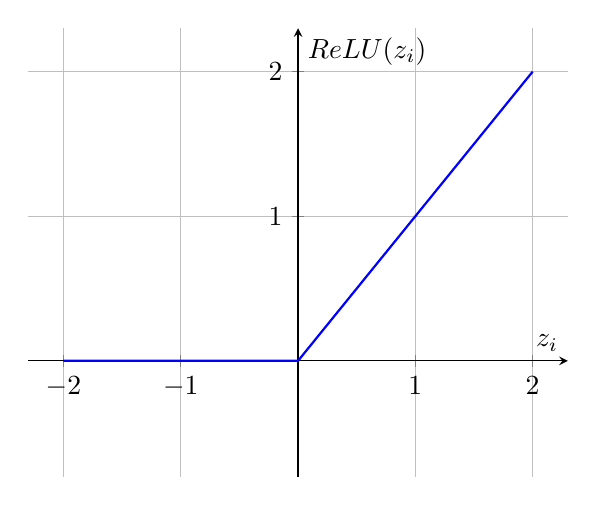
\begin{tikzpicture}
            \begin{axis}[
                xlabel={$z_i$},
                ylabel={$\text{ReLU}(z_i)$},
                xmin=-2.3, xmax=2.3,
                ymin=-0.8, ymax=2.3,
                axis lines=middle,
                grid=major,
            ]
            \addplot[blue, thick, domain=-2:2] {max(0, x)};
            \end{axis}
        \end{tikzpicture}
        \label{fig:relu}
\end{figure}

Como estamos trabalhando com redes neurais, uma das maiores vantagens dessas redes é o fato delas “aprenderem” com base na retropropagação do gradiente nas camadas da rede. Assim, ao calcularmos o gradiente para fazer a retropropagação do erro e ajustar os pesos e vieses das camadas, é necessário ter em mente também a derivada daquela função de ativação que vamos aplicar em uma camada de neurônios da rede, dado que ela entrará no backward pass do modelo.

Para achar a derivada da ReLU, podemos simplesmente derivar as duas condicionais dela, assim, quando $x$ for maior que zero, a saída será 1, já quando $x$ for menor que zero, a saída será zero. Mas encontramos um problema nisso, a derivada dessa função não existe quando $x$ é 0, pois o limite lateral à esquerda dessa função é zero, enquanto o limite lateral a direita dela é um. Isso passa a ser um problema quando queremos calcular o valor de saída justamente quando aquele valor de entrada é zero. Na prática, esse problema é fácil de resolver quando estamos trabalhando com o código dessa função, basta escolhermos qual será o resultado da ReLU quando esse valor de entrada for zero. Podemos dizer que ele será 1 ou zero, isso irá depender somente da nossa implementação da derivada da ReLU. Note que, essa descontinuidade da ReLU, se torna um problema quando estamos trabalhando com sua derivada.

Assim, temos a equação \ref{eq:relu-derivada}.

\begin{equacaodestaque}{Derivada Rectified Linear Unit (ReLU)}
    \frac{d}{dz_i} [ReLU](z_i) = \begin{cases}1, & \text{se } z_i > 0 \\0, & \text{se } z_i \leqslant 0 \end{cases}
    \label{eq:relu-derivada}
\end{equacaodestaque}

Esse detalhe da descontinuidade da ReLU no ponto zero foi algo que acabou mudando em funções futuras, que buscam corrigir erros da ReLU e melhorá-la,assim, com o passar do tempo foram surgindo outras alternativas que também trabalhassem com os atributos da ReLU, mas que fossem contínuas em toda a reta, permitindo a sua derivação também em todos os pontos. Uma dessas funções a ELU, ela será explicada mais em frente.

Além de termos a sua derivada em equação, podemos fazer também o seu gráfico na figura \ref{eq:relu-derivada}, note que ela é ainda mais simples que a própria função de ativação, são só duas retas constantes que irão retornar zero quando o número for menor que zero, ou irão retornar 1 quando a entrada for um número maior que zero.

\begin{figure}[h!] % Use [htbp] para dar flexibilidade ao LaTeX
    \centering % Centraliza o gráfico na página
    \caption{Gráfico da Derivada da Função ReLU}
    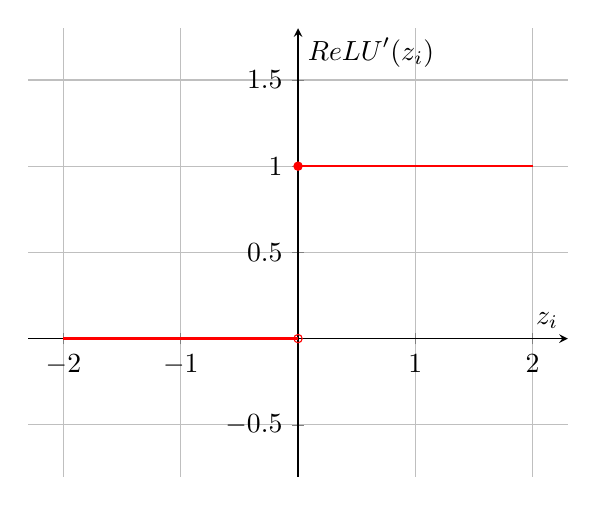
\begin{tikzpicture}
        \begin{axis}[
            xlabel={$z_i$},
            ylabel={$\text{ReLU}'(z_i)$},
            xmin=-2.3, xmax=2.3,
            ymin=-0.8, ymax=1.8,
            axis lines=middle,
            grid=major
        ]
        \addplot[red, thick, domain=-2:0] {0};
        \addplot[red, thick, domain=0:2] {1};
        \addplot[red, only marks, mark=o, mark size=1.5pt] coordinates {(0,0)};
        \addplot[red, only marks, mark=*, mark size=1.5pt] coordinates {(0,1)};
        \end{axis}
    \end{tikzpicture}
    \label{fig:relu-derivada}
\end{figure}

Assim, conhecemos a ReLU, uma função que é considerada padrão para a maioria das redes neurais \textit{feedforward} \parencite{DeepLearningBook}. Vimos que ela veio para ser uma alternativa para as funções sigmoides, sendo mais simples e resolvendo o problema do gradiente em fuga, contudo, a ReLU também apresenta problemas, como o do neurônios agonizantes a o explosão de gradientes, uma versão diferente do problema do gradiente em fuga. Dito isso, eles serão explicados em seguida para entendermos também as desvantagens de se utilizar essa função em uma rede neural.

\subsection{Implementação em Python}

Agora que sabemos qual é o comportamento da ReLU, quais são suas fórmulas e quais são seus gráficos, podemos trabalhar em uma implementação dessa função utilizando Python. Para fazer isso, vamos criar uma classe, com duas funções: a \textit{forward} e a \textit{backward}. A função \textit{forward} é responsável por implementar a ReLU, já a \textit{backward} implementa a sua derivada. Para criar a \textit{forward}, podemos utilizar uma função já pronta da biblioteca numpy, a maximum, essa função é responsável por comparar dois valores e escolher o maior deles. Neste caso, um dos valores será sempre zero, enquanto o outro será a entrada da função. Já a \textit{backward}, irá receber o gradiente retropropagado, e irá aplicar na fórmula da derivada da ReLU, comparando se aquele valor é negativo e retornando zero, caso for, ou um caso seja positivo.

\textbf{Implementação em Python}

\begin{codelisting}{Classe completa do função de ativação Rectified Linear Unit}{gd_class}
import numpy as np
from layers.base import Layer

class ReLU(Layer):
    def __init__(self):
        super().__init__()
        self.input = None

    def forward(self, input_data):
        self.input = input_data
        return np.maximum(0, self.input)

    def backward(self, grad_output):
        relu_grad = (self.input > 0)

        # Apply the chain rule
        return grad_output * relu_grad, None
\end{codelisting}

\section{Dying ReLUs Problem}

\section{Corrigindo o Dying ReLUs Problem: As Variantes com Vazamento}

Diferente da ReLU tradicional que retorna zero para os casos em que sua entrada é negativa e por isso na sua derivada irá também retornar zero nestes casos, as variantes com vazamento atuam de outra forma, elas retornam um valor muito pequeno como 0.1, multiplicado pela entrada da função quando ela é negativa. Por isso, a sua derivada será algo também 0.1 (ou valores muito pequenos), isso permite um "vazamento" do gradiente em cenários nos quais a entrada do neurônio será negativa.

Nós vimos, que a causa do neurônios agonizantes era justamente isso: muitas situações em que a entrada era negativa, que gerava um gradiente nulo e consequentemente impedia os neurônios de terem seus pesos e vieses ajustados, e futuramente morrendo, retornando zero independente de qual fosse a sua entrada.

Assim, essas variantes, como a Leaky ReLU e a PReLU buscam tentar corrigir um amenizar esse problema da ReLU mas mantendo algumas de suas principais propriedades, como a não linearidade, a capacidade de ser escrita compondo duas retas permitindo a criação de uma função simples e rápida de ser computada em uma rede neural.

\subsection{Leaky ReLU (LReLU)}

Seguindo adiante, a próxima função que iremos ver é a Leaky ReLU, ela é uma variante da ReLU que foi criada com intuito de corrigir o problema do neurônios agonizantes. Assim como a ReLU, que foi explicada com a analogia do vendedor de pipoca, podemos extender essa explicação para essa nova função, antes o limiar para comprar um pacote de pipoca era de R\$ 5,00, quem tivesse menos que isso não comprava nada. Mas agora, para garantir que todos possam comprar pipoca, você como vendedor definiu que quando uma pessoa tiver menos que R\$ 5,00 ela também será capaz de comprar pipoca, só que neste caso ela comprará um punhado de pipoca que será proporcional ao dinheiro que ela tem multiplicado por uma constante $\alpha$. Assim, uma pessoa com um valor próximo de R\$ 5,00 pode sair com um punhado de pipoca quase igual ao do pacote original se essa constante $\alpha$ for um valor muito proximo de um. Com isso, você como vendedor consegue obter lucro com uma nova clientela além de não perder clientes por não possuírem o valor total do pacote de pipoca. A Leaky ReLU traz uma proposta parecida para resolver com o problema do neurônios agonizantes.

Ela foi apresentada no artigo \textit{Recfier Nonlinearites Improve Neural Networks Acustic Models}, em que os autores exploram o uso de redes retificadoras profundas como modelos acústicos para a tarefa de reconhecimento de fala conversacional \textit{switchboard} \parencite{LeakyReLUArticle}. Além disso, a sua principal diferença, como explicam \textcite{LeakyReLUArticle}, está no fato dela permitir que um pequeno gradiente diferente de zero flua quando a unidade está saturada e não ativa. Esse gradiente diferente de zero que flui quando a unidade está saturada e não ativa são os seus compradores de pipoca que não possuem o valor total mas são capazes de comprar um punhado dela, neste caso a unidade estará não ativa pois o valor de entrada é negativo mas irá retornar um valor diferente de zero, algo que não acontecia na ReLU.

Seguindo adiante, podemos discutir a expressão matemática da Leaky ReLU, a qual é dada pela equação \ref{eq:leaky-relu}, que é bem parecida com a ReLU, porém, ela também irá retornar valores negativos quando a sua entrada for um valor negativo, diferente da ReLU, que iria retornar como saída zero. A constante $\alpha$, no texto original é dada por 0.1 fazendo com que os valores negativos sejam pequenos mas ainda sim, diferentes de zero quando passam pela entrada \parencite{LeakyReLUArticle}. Cabe destacar que, essa constante $\alpha$ pode ser ajustada para diferentes cenários, podendo ser valores diferentes de 0.1 como foram propostos no texto original, é possível ver isso acontecendo em comparativos ao longo desse texto, em que diferentes autores optam por valores diferentes de $\alpha$ para melhor ajustar ao problema que está sendo analisado.

\begin{equacaodestaque}{Leaky ReLU (LReLU)}
    \text{LReLU}(z_i) = \begin{cases}z_i, & \text{se } z_i \ge 0 \\ \alpha \cdot z_i, & \text{se } z_i < 0\end{cases} \text{ou} \text{LReLU}(z_i) = \max(0, \alpha z_i)
    \label{eq:leaky-relu}
\end{equacaodestaque}

Já para a sua representação gráfica, podemos plotar o seu gráfico na figura \ref{fig:leaky-relu}, analisando ele, vemos que a Leaky ReLU possui características muito semelhantes com a ReLU, como o fato dela assumir o comportamento de uma função identidade para para valores positivos em sua entrada, mas, quando analisamos seus valores negativos vemos uma diferença, agora eles são dados por um gráfico de uma função do primeiro grau, diferente da ReLU que era uma função constante em zero. Além disso, a LReLU, também é uma função assimétrica e não linear, bem como apresenta um ponto de descontinuidade em zero, pois ao traçarmos os seus limites laterais, eles apresentam valores diferentes, por isso ela não pode ser derivada nesse ponto, assim como a ReLU que vimos anteriormente.

\begin{figure}[h!]
    \centering
    \caption{Gráfico da Função Leaky ReLU (LReLU) com $\alpha = 0.1$}
    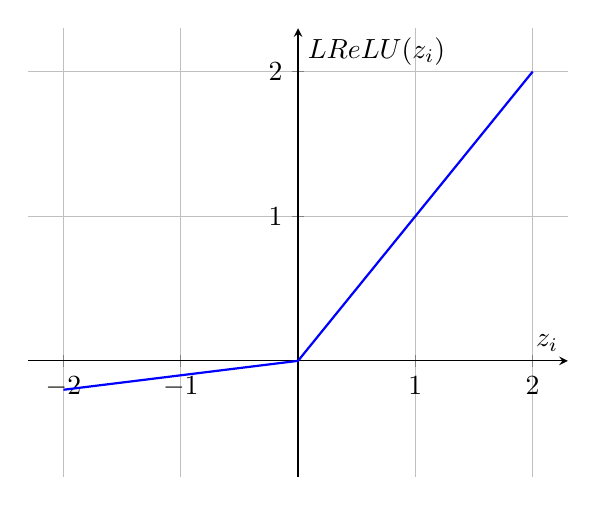
\begin{tikzpicture}
        \begin{axis}[
            xlabel={$z_i$},
            ylabel={$\text{LReLU}(z_i)$},
            xmin=-2.3, xmax=2.3,
            ymin=-0.8, ymax=2.3,
            axis lines=middle,
            grid=major,
        ]
        % \leakyalpha é o comando que você definiu no preâmbulo (0.1)
        \addplot[blue, thick, domain=-2:2] {x > 0 ? x : 0.1*x};
        \end{axis}
    \end{tikzpicture}
    \label{fig:leaky-relu}
\end{figure}

Sabendo de sua expressão e seu gráfico, podemos nos preocupar agora a calcular sua derivada, para isso, devemos derivar as duas condicionais que estão na função da Leaky ReLU. Assim, quando a entrada dessa função for maior que zero, essa função será $x$ que derivada é 1, já quando a entrada for menor que zero, a função será $\alpha x$, que quando derivada tem como resultado a própria constante $\alpha$. Contudo, como dito anteriormente, a derivada da Leaky ReLU não existe quando a entrada é exatamente zero, mas na prática, quando estamos trabalhando com a sua definição na retropropagação, podemos definir um valor para a derivada nesse ponto, assim como fizemos com a ReLU tradicional. Com isso em mente, temos a equação \ref{eq:leaky-relu-derivada} que representa a derivada da Leaky ReLU, note que para a sua derivada nós não temos uma expressão reduzida quando comparada com a expressão original.

\begin{equacaodestaque}{Derivada Leaky ReLU (LReLU)}
    \frac{d}{dz_i} [LReLU](z_i) = \begin{cases}1, & \text{se } z_i > 0 \\ \alpha, & \text{se } z_i \leqslant  0 \end{cases}
    \label{eq:leaky-relu-derivada}
\end{equacaodestaque}

Já que agora conhecemos a sua derivada, podemos também plotar o seu gráfico, o qual é dado pela figura \ref{fig:leaky-relu-derivada}. Ele também é parecido com o gráfico da ReLU que vimos anteriormente, sendo composto por duas retas constantes, para valores positivos ele retorna 1 (assim como a ReLU), e para valores negativos ou nulos ele irá sempre retornar a constante $\alpha$, diferente da ReLU, que iria retornar zero, indicando que neste caso o neurônio não está passando nenhuma informação na na retropropagação do gradiente. Por esse motivo que e a Leaky ReLU tem esse nome, pois leaky em inglês significa "vazamento", e neste caso, como a derivada dela é diferente de zero, mesmo quando a entrada for negativa, ela irá passar informações durante a retropropagação, isso permite que o neurônio não morra, como acontecia em algumas redes que faziam uso da ReLU tradicional, e por esse motivo continue aprendendo pelo fato do gradiente continuar fluindo pela rede e consequentemente atualizando os pesos e vieses dos neurônios.

\begin{figure}[h!]
    \centering
    \caption{Gráfico da Derivada da Função Leaky ReLU (LReLU) com $\alpha = 0.1$}
    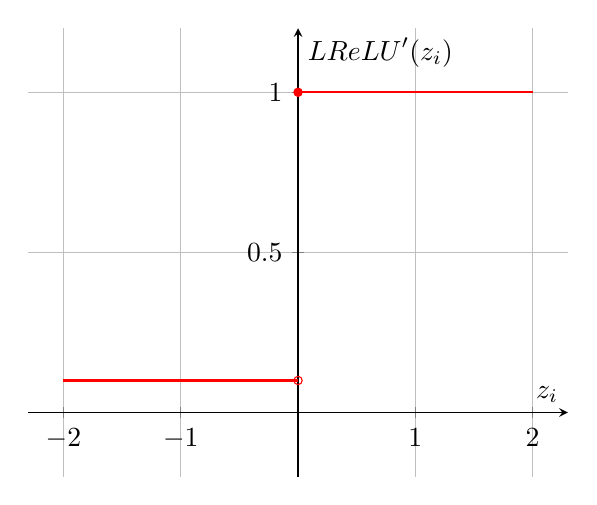
\begin{tikzpicture}
        \begin{axis}[
            xlabel={$z_i$},
            ylabel={$\text{LReLU}'(z_i)$},
            xmin=-2.3, xmax=2.3,
            ymin=-0.2, ymax=1.2,
            axis lines=middle,
            grid=major
        ]
        \def\alphaVal{0.1} % Define alpha for the derivative graph

        \addplot[red, thick, domain=-2:0] {\alphaVal};
        \addplot[red, thick, domain=0:2] {1};
        \addplot[red, only marks, mark=o, mark size=1.5pt] coordinates {(0,\alphaVal)};
        \addplot[red, only marks, mark=*, mark size=1.5pt] coordinates {(0,1)};
        \end{axis}
    \end{tikzpicture}
    \label{fig:leaky-relu-derivada}
\end{figure}

Voltando para \textit{Recfier Nonlinearites Improve Neural Networks Acustic Models}, \textcite{LeakyReLUArticle} explicam sobre outras propriedades da LReLu, como o fato dela sacrificar a esparsidade de zero duros (\textit{hard-zero sparsity}) para ter um gradiente  que é potencialmente mais robusto durante a otimização da rede neural. Além disso, os autores também explicam que ambas as funções retificadoras, tanto a ReLU quando a Leaky ReLU se saem bem nos testes de performance quando comparadas com a tangente hiperbólica além de se beneficiarem melhor da profundidade de rede quando comparadas com as sigmoides \parencite{LeakyReLUArticle}.

Em testes de desempenho realizados por \textcite{LeakyReLUArticle}, eles foram capazes de analisar como uma rede neural que faz uso dessa função pode performar quando comparada com a ReLU tradicional e também com redes que fazem uso da Tangente hiperbólica, esse comparativo pode ser visto na tabela \ref{tab:lrelu_desempenho_apa}. Nós podemos nessa tabela que as redes neurais que fizeram uso da Leaky ReLU como função de ativação obtiveram melhores resultandos quando comparadas com as redes que utilizaram a ReLU tradicional ou  a Tangente Hiperbólica, vemos que a rede que foi construída com 3 camadas utilizando a LReLU foi capaz de obter a taxa de erro de palavra (WER) mais baixa no conjunto SWBD, com 17.8\%, esse resultado 0.3 pontos percentuais menor quando comparado com uma mesma rede de três camadas que utilizou a ReLU tradicional.

Além disso, ainda na \ref{Tab:leaky-relu-desempenho}, nas redes compostas por três camadas, a rede que fez uso da LReLU também foi melhor que suas outras concorrentes que fizeram uso da ReLU e da tanh, sendo capaz de ter a menor taxa de erro de palavra no conjunto de avaliação (EV), com 24.3\%, uma diferença de 0.1 pontos percentuais quando comparada com a ReLU de 24.4\%, já quando essa rede é comparada com a tangente hiperbólica, a diferença é ainda maior, sendo de 2.1 pontos percentuais, indicando que a LReLU trás resultados melhores quando comparada com essas duas funções de ativação.

\begin{table}[ht]
    \caption{Comparativo de Desempenho de Redes Neurais para Reconhecimento de Fala}
    \label{tab:leaky-relu-desempenho}
    \centering
    \begin{tabular}{lccccc}
        \toprule
        \textbf{Modelo} & \textbf{Dev CrossEnt} & \textbf{Dev Acc (\%)} & \textbf{SWBD WER} & \textbf{CH WER} & \textbf{EV WER} \\
        \midrule
        
        GMM Baseline & N/A & N/A & 25.1 & 40.6 & 32.6 \\ 
        \addlinespace % Adiciona um espaço para separar o baseline dos outros
        2 Camadas Tanh  & 2.09 & 48.0 & 21.0 & 34.3 & 27.7 \\
        2 Camadas ReLU  & 1.91 & 51.7 & 19.1 & 32.3 & 25.7 \\
        2 Camadas LReLU & 1.90 & 51.8 & 19.1 & 32.1 & 25.6 \\ 
        \addlinespace
        3 Camadas Tanh  & 2.02 & 49.8 & 20.0 & 32.7 & 26.4 \\
        3 Camadas ReLU  & 1.83 & 53.3 & 18.1 & 30.6 & 24.4 \\
        3 Camadas LReLU & 1.83 & 53.4 & \textbf{17.8} & 30.7 & \textbf{24.3} \\ 
        \addlinespace
        4 Camadas Tanh  & 1.98 & 49.8 & 19.5 & 32.3 & 25.9 \\
        4 Camadas ReLU  & 1.79 & 53.9 & 17.3 & 29.9 & 23.6 \\
        4 Camadas LReLU & \textbf{1.78} & 53.9 & 17.3 & 29.9 & 23.7 \\
        
        \bottomrule
    \end{tabular}
    \vspace{2mm}
    
    \parbox{\linewidth}{\small
        \textit{Nota.} Comparação de métricas de erro para sistemas de redes neurais profundas (DNN) em reconhecimento de fala. As métricas de quadro a quadro (frame-wise) foram avaliadas em um conjunto de desenvolvimento, e as taxas de erro de palavra (WER) no conjunto de avaliação Hub5 2000 e seus subconjuntos. Abreviações: Dev CrossEnt = Entropia Cruzada no conjunto de desenvolvimento; Dev Acc = Acurácia no conjunto de desenvolvimento; WER = Taxa de Erro de Palavra (Word Error Rate); SWBD = Switchboard; CH = CallHome; EV = Evaluation set. Valores em negrito indicam os melhores resultados para modelos de 3 e 4 camadas.
        Adaptado de "Rectifier Nonlinearities Improve Neural Network Acoustic Models", por A. L. Maas, A. Y. Hannun, \& A. Y. Ng, 2013, \textit{In Proceedings of the 30th International Conference on Machine Learning, Workshop on Deep Learning for Audio, Speech and Language Processing}.
    }
\end{table}

Agora comparando as redes que fazem uso de quatro camadas, cabe destacar os resultados da entropia cruzada no conjunto de desenvolvimento (Dev CrossEnt), que é uma métrica responsável por medir a diferença entre duas distribuições de probabilidade, neste cenário: a distrubição de probabilidade prevista pelo modelo e a distribuição de probabilidade real, com base nesses dois valores, a entropia cruzada consegue medir o quão bem o modelo de rede neural criado pelos pesquisadores está prevendo a transcrição correta da fala durante a fase de treinamento e ajuste, para isso, é utilizado o conjunto de dados de desenvolvimento (Dev Set). Tendo isso em mente, o modelo de quatro camadas que fez uso da Leaky ReLU em sua arquitetura obteve o melhor resultado dos seus outros dois concorrentes, para isso, sendo assim, ele teve como resultado uma entropia cruzada de 1.78, 0.01 menor que o modelo que fez uso da ReLU tradicional (que obteve 1.79) e 0.2 menor que o modelo que fez uso da tangente hiperbólica (que obteve 1.98).

Ainda no grupo de redes que possuem quatro camadas, podemos ver um empate quando analisamos a acurácia no conjunto de desenvolvimento (Dev Acc), que é uma métrica responsável por medir a proporção das previsões corretas feitas pelo modelo quando comparadas com o total de previsões feitas. Assim, quando vemos a tabela \ref{tab:lrelu_desempenho_apa}, as redes que fizeram uso tanto da ReLU quanto da Leaky ReLU obtiveram a mesma acurácia de 53.9\%, já quando comparamos com a tangente hiperbólica, vemos uma diferença de 4.1 pontos percentuais, indicando as funções retificadoras acabam sendo mais precisas para essa análise. Não somente elas são mais precisas, mas quando comparamos com a Leaky ReLU, vemos outros ganhos também, como menores taxas de erro de palavra (WER) tanto no conjunto Switchboard (SWBD) quanto no conjunto de avaliação (EV).

A Leaky ReLU já é uma evolução quando comparamos com a ReLU tradicional, mas, podemos ir além e encontrar funções ainda mais complexas que também buscam assim como a LReLU resolver o problema do neurônios agonizantes com um vazamento de gradiente nos casos negativos, uma dessas funções é a PReLU, a qual veremos em seguida.

\textbf{Implementação em Python}

\begin{codelisting}{Classe completa do função de ativação Leaky ReLU}{gd_class}
import numpy as np
from layers.base import Layer


class LeakyReLU(Layer):
    def __init__(self, alpha=0.01):
        super().__init__()
        self.input = None
        self.alpha = alpha

    def forward(self, input_data):
        self.input = input_data
        return np.maximum(self.input * self.alpha, self.input)

    def backward(self, grad_output):
        leaky_relu_grad = np.where(self.input > 0, 1, self.alpha)
        return grad_output * leaky_relu_grad, None
\end{codelisting}

\subsection{Parametric ReLU (PReLU)}

Continuando nas analogias do vendedor de pipoca para explicar as funções retificadoras, podemos também pensar uma para a Parametric ReLU. Na LReLU nós tínhamos uma constante fixa, que valia para todos os valores de entrada e não mudava, era como se o vendedor de pipoca definisse um valor para a proporção de pipoca que a pessoa irá receber quando tiver com uma quantia menor de dinheiro que o limiar da venda. Mas agora, este vendedor está mais experiente, e sabe que pode ajustar essa constante sempre que quiser, assim, quando estiverem muitas pessoas na praça em que está vendendo pipoca, ele poderá colocar uma constante que será capaz de dar uma quantidade ainda maior de pipoca para aqueles que não possuem o valor total de um pacote, o que incentivaria a venda para as pessoas. Já quando estivesse em um lugar mais vazio, colocaria uma constante que daria menos pipoca, para maximizar o seu lucro. A Diferença da PReLU para a LReLU está justamente nessa constante e como ela irá se comportar.

Proposta por \textcite{PReLUArticle} no artigo \textit{Delving Deep into Rectifiers: Surpassing Human Level Performance on Image Net Classification}, a PReLU surgiu como uma variação não somente da ReLU, mas também uma evolução da Leaky ReLU que vimos anteriormente, isso ocorre, pois diferente da LReLU que possuía uma constante $\alpha$ fixa que multiplicava o valor da entrada nos casos negativos, a PReLU trás essa mesma constante, mas neste caso ela é adaptável, se ajustando as particularidades de cada problema que uma rede neural está tentando resolver. Assim, a PReLU é como o pipoqueiro mais experiente, que ajusta como vai vender o seu punhado de pipoca em cada uma das situações para poder maximizar os seus lucros mas ao mesmo tempo garantir mais clientes para si.

Agora que conhecemos a Parametric ReLU e sabemos de seu potencial, podemos estudar a sua fórmula matemática, a qual é dada pela expressão \ref{eq:prelu}. Como explicam \textcite{PReLUArticle}, a PReLU generaliza a tradicional ReLU, além de melhorar o \textit{model fitting} apresentando quase nenhum custo computacional extra e com um baixo risco de sobreajuste (\textit{overfitting}). Este coeficiente $\alpha$, que ela apresenta assim como a Leaky ReLU que vimos anteriormente, é aprendível, e não uma constante fixa, isso indica ser otimizado utilizando a retropropagação do gradiente de forma simultânea com as outras camadas da rede neural criada \parencite{PReLUArticle}. Assim, por esse fato temos uma melhor eficiência no aprendizado e no tempo da rede, dado que não precisamos criar uma nova etapa só para ajustar os valores de alpha das camadas densas que fazem o uso da Parametric ReLU.

\begin{equacaodestaque}{Parametric ReLU (PReLU)}
    \text{PReLU}(z_i) = \begin{cases}z_i, & \text{se } z_i \ge 0 \\ \alpha_i \cdot z_i, & \text{se } z_i < 0\end{cases} \text{ou} \text{PReLU}(z_i) = \max(0, \alpha z_i)
    \label{eq:prelu}
\end{equacaodestaque}

Com base em sua equação, podemos plotar o gráfico da PReLU na figura \ref{fig:prelu}, note que caso este coeficiente for igual a zero, nos temos então a ReLU tradicional, já quando ele for igual a 0.1, teremos a LReLU, no gráfico $\alpha$ está com valor de 0.2, mas ele irá variar conforme a rede aprende e para cada problema, podendo apresentar diferentes valores em diferentes situações. Com isso, nos notamos que a PReLU é composta por duas funções do primeiro grau, sendo assimétrica, e também apresentando um ponto de descontinuidade em zero, o que impede de ser derivada neste ponto.

\begin{figure}[h!]
    \centering
    \caption{Gráfico da Função Parametric ReLU (PReLU) com $\alpha=0.2$}
    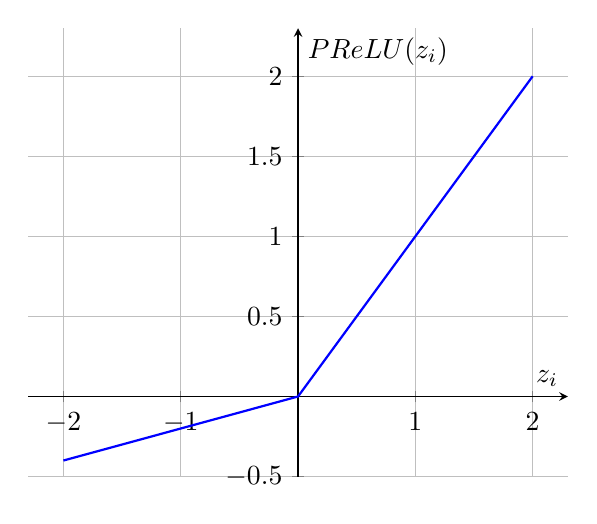
\begin{tikzpicture}
        \begin{axis}[
            xlabel={$z_i$},
            ylabel={$\text{PReLU}(z_i)$},
            xmin=-2.3, xmax=2.3,
            ymin=-0.5, ymax=2.3,
            axis lines=middle,
            grid=major,
        ]
        % Define um valor exemplo de alpha para o gráfico
        \def\alphaVal{0.2} 
        \addplot[blue, thick, domain=-2:2] {x >= 0 ? x : \alphaVal*x};
        \end{axis}
    \end{tikzpicture}
    \label{fig:prelu}
\end{figure}

Se conhecemos a sua fórmula e como ela se comporta, podemos também derivar a PReLU, para isso, derivamos cada uma das expressões dos condicionais de forma separada, assim como fizemos com a Leaky ReLU e a ReLU anteriormente. Como a fórmula da PReLu é igual a LReLU, podemos apenas nos lembrar dela e citar a expressão \ref{eq:prelu-derivada} como sua derivada. Note que, essa derivada também não existe quando a entrada é exatamente zero, mas assim como na Leaky ReLU, "corrigimos" isso dizendo que ela será igual a $\alpha$ nesse ponto, para que o gradiente continue fluindo durante o backward pass. Vale lembrar, que essa reta em $\alpha$ irá variar conforme a rede neural aprende as características e se ajusta ao problema que está tentando resolver.

\begin{equacaodestaque}{Derivada Parametric ReLU (PReLU)}
    \frac{d}{dz_i} [PReLU](z_i) = \begin{cases}1, & \text{se } z_i > 0 \\ \alpha_i, & \text{se } z_i < 0 \\ \nexists, & \text{se } z_i = 0\end{cases}
    \label{eq:prelu-derivada}
\end{equacaodestaque}

Sabendo a fórmula da derivada da PReLU, podemos também plotar o seu gráfico, o qual é dado pela figura \ref{fig:prelu-derivada}, ele é semelhante ao gráfico da Leaky ReLU visto na seção anterior, mas agora, a constante $\alpha$ está com valor em 0.2. Note que, o gráfico da derivada é também muito simples, sendo apenas duas funções constantes, uma que vale 1 para os valores de entrada positivos e outra que irá valer 0,2 para os outros valores. Assim, a PReLU consegue manter a simplicidade da ReLU, mas ao mesmo tempo fazendo pequenos ajustes garantindo melhorias de desempenho em redes mais profundas, como as que vimos apresentas por \textcite{PReLUArticle}.

\begin{figure}[h!]
    \centering
    \caption{Gráfico da Derivada da Função Parametric ReLU (PReLU) com ($\alpha=0.2$)}
    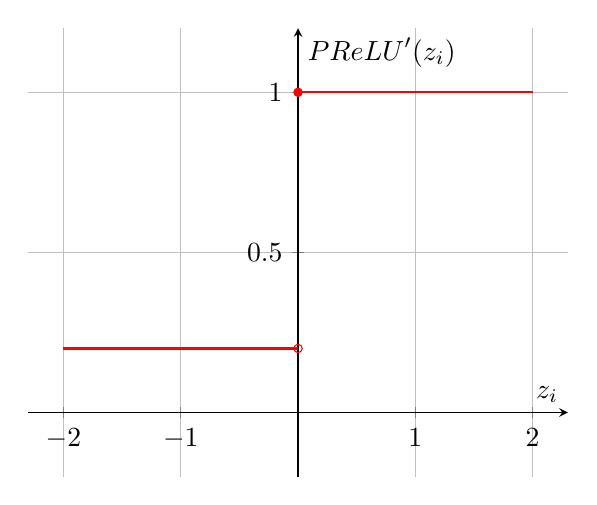
\begin{tikzpicture}
        \begin{axis}[
            xlabel={$z_i$},
            ylabel={$\text{PReLU}'(z_i)$},
            xmin=-2.3, xmax=2.3,
            ymin=-0.2, ymax=1.2,
            axis lines=middle,
            grid=major
        ]
        % Define um valor exemplo de alpha para o gráfico
        \def\alphaVal{0.2}

        \addplot[red, thick, domain=-2:0] {\alphaVal};
        \addplot[red, thick, domain=0:2] {1};
        \addplot[red, only marks, mark=o, mark size=1.5pt] coordinates {(0,\alphaVal)};
        \addplot[red, only marks, mark=*, mark size=1.5pt] coordinates {(0,1)};
        \end{axis}
    \end{tikzpicture}
    \label{fig:prelu-derivada}
\end{figure}

Ainda em \textit{Delving Deep into Rectifiers: Surpassing Human Level Performance on Image Net Classification}, os autores realizam testes comparando a ReLU tradicional com a PReLU utilizando como base o dataset de 1000 classes do ImageNet 2012, o qual contêm cerca de 1.2 milhões de imagens de treino, 50.000 imagens de validação e 100.000 imagens de teste sem rótulos publicados \parencite{PReLUArticle}. Para isso, \textcite{PReLUArticle} criaram três modelos diferentes (A, B e C), baseados na arquitetura VGG-16 mas com variações entre si como diferentes números de camadas convolucionais e consequentemente complexidades distintas para cada algoritmo. Esses modelos podem ser vistos na tabela \ref{tab:arquitetura_prelu}. 

Conhecendo cada um dos modelos apresentados por \textcite{PReLUArticle}, podemos analisar como eles se comportaram nos testes de performance utilizando o dataset do ImageNet 2012, para isso, os autores realizaram testes tanto utilizando a nova função de ativação PReLU, mas também a ReLU tradicional, podendo ter uma base melhor para suas comparações. Além disso, como podemos ver na tabala \ref{tab:prelu_desempenho1}, é medido o erro Top-1 e o erro Top-5, o erro Top-1 nos mostra quão preciso é o modelo em seu melhor chute, já o erro Top-5 nos mostra se a resposta correta estava entre os top 5 melhores chutes feito pelo modelo. Assim, conhecendo esses parâmetros de medida, podemos chegar na conclusão de que quanto menor esses valores, melhor o modelo está performando, seguindo essa lógica, podemos ver que todos os modelos que fazem uso de funções retificadoras, seja a PReLU ou mesmo a ReLU tradicional, são capazes de performar melhor que os modelos VGG-16 e GoogleLet que fazem uso de outras funções de ativação.

Quando comparamos o modelo C, que faz uso da PReLU e possui mais camadas convolucionais, com o modelo A que faz uso da ReLU, vemos uma diferença de 2,21 pontos percentuais no erro Top-1, já quando analisamos o erro Top-5, essa diferença é de 1,21 pontos percentuais, o que indica que a ReLU é capaz de trazer melhores resultados quando comparada com redes que fazem uso da ReLU tradicional. Já quando comparamos com o VGG-16, essa diferença de desempenho é ainda maior, sendo de 3,8 pontos percentuais no erro Top-1 e 1,95 pontos percentuais no erro Top-5, note que a VGG-16, a qual é indicada na tabela \ref{tab:arquitetura_prelu} possui bem menos camadas convolucionais que o modelo C, podemos notar também a sua complexidade computacional, que é menos da metade da do modelo C, isso indica que a PReLU, por ser uma função não saturante e consequentemente corrigir o problema do gradiente em fuga, é capaz de criar redes neurais que se beneficiam melhor com uma maior profundidade, sendo capazes de extrair mais informações e com isso performar melhor.

Um feito importante que deve ser destacado sobre a PReLU, que inclusive é o nome do artigo que foi responsável por introduzir essa função para a comunidade científica, é de que durante a pesquisa do texto \textit{Delving Deep into Rectifiers: Surpassing Human Level Performance on Image Net Classification}, \textcite{PReLUArticle} foram capazes de criar uma rede neural capaz de superar a capacidade humana de reconhecer diferentes conjuntos de imagens no ImagneNet Classification, isso ocorreu porque a um humano ao analisar o ImageNet apresenta uma taxa de erro Top-5 de 5.1\% e em um dos testes realizados pelos autores, uma rede neural alcançou uma taxa de erro Top-5 de 4.94\%, superando assim a capacidade humana de reconhecimento de imagens. 

Assim, é nítido destacar que não somente a PReLU, mas as funções retificadoras de forma geral, foram capazes de trazer melhorias significativas para os modelos de aprendizado profundo quando comparadas com as funções sigmoides, as quais foram o padrão da indústria por muitos anos. De fato, a resolução do problema do gradiente em fuga, possibilitou a criação de redes neurais ainda mais profundas, e com isso, sendo capazes de extrair mais informações e consequente melhores métricas, sendo capazes até de superar a capacidade humanas em algumas tarefas como nós vimos no texto.

\textbf{Implementação em Python}

\subsection{Randomized Leaky ReLU}

Anteriormente, na Parametric ReLU, nós tínhamos uma padrão aprendível que era atualizado ao longo da retropropagação da rede, nós o comparamos com o caso do vendedor de pipoca ficando mais experiente para as vendas. No caso da RReLU temos um vendedor um tanto quanto instável, ele se baseia na sorte/aleatoriedade para definir qual será o punhado de pipoca que cada pessoa irá receber ao comprar com um valor abaixo do limiar de venda. Para isso, não existe mais um padrão, algo como o horário ou a quantidade de pessoas na praça para fazer aumentar o diminuir a quantidade de pipoca que tera em um punhado. Essa estratégia parece caótica, mas pode ser interessante caso voce queira instigar as vendas e deixa-las divertidas, você pode comprar um punhado de pipoca, mas nao ira saber quanto irá receber, é uma grande aposta.

Segundo \textcite{XuRReLU}, em \textit{Empirical Evaluation of Rectified Activations in Convolutional Network}, a Randomized Leaky ReLU foi proposta pela primeira vez em uma competição do Kaggle NDSB, ela era uma função semelhante a leaky ReLU mas que o seu coeficiente $\alpha$ é um número aleatório dado pela distribuição normal da forma $U(l, u)$, nessa mesma competição os valores escolhidos para essa distribuição foram de $U(3, 8)$.

Agora que entendemos um pouco de como a Randomized Leaky ReLU funciona, podemos entender melhor a sua fórmula, a qual é dada pela expressão \ref{eq:rrelu}, note que é a mesma expressão da Leaky ReLU e da PReLU, mas o que muda é o significado do termo $\alpha$ em cada uma delas. Neste caso temos que $\alpha \sim U (l, u)$ em que $l < u$  e $l, u \in [0, 1)$ 

\begin{equacaodestaque}{Randomized Leaky ReLU (RReLU)}
    \text{RReLU}(z_i) = \begin{cases} z_i, & \text{se } z_i > 0 \\ \alpha_i z_i, & \text{se } z_i \leq 0 \end{cases}
    \label{eq:rrelu}
\end{equacaodestaque}

Na fase de testes, devemos calcular a média de todos os valores de $\alpha$ durante o treino, e com isso $\alpha$ se torna uma constante fixa do tipo $(l+u)/2$ de forma que com isso seja possível obter um resultado determinístico, no artigo, os autores utilizam a fórmula \ref{eq:EquacaoRReLU2} para calcular a RReLU durante o teste do modelo \parencite{XuRReLU}.

Conhecendo como a Randomized Leaky ReLU se comporta, podemos plotar o seu gráfico, o qual está presente na figura \ref{fig:rrelu}. Na representação, é possível ver várias retas, isso ocorre pois elas irão variar de caso a caso, e como a RReLU é uma função que utiliza de conceitos probabilísticos, não podemos garantir um gráfico exato de como ela seria pois não temos os valores de $\alpha$ até que a distribuição seja feita. Note que mesmo com essa particularidade, ela ainda continua sendo uma função bem simples, sendo a construção de duas retas originarias de equações do primeiro grau, a primeira delas sendo a própria função identidade, para os casos em que a entrada é positiva, e a outra é dada pela variável da entrada multiplicada pela constante $\alpha$, para os casos em que a saída é negativa. Além disso, devemos nos atentar também para a sua descontinuidade no ponto zero, é o mesmo problema que acontece com outras variantes, como a ReLU e a Leaky ReLU.

\begin{figure}[h!]
    \centering
    \caption{Gráfico da Função Randomized Leaky ReLU (RReLU) com Diferentes Inclinações Aleatórias para a Parte Negativa}
    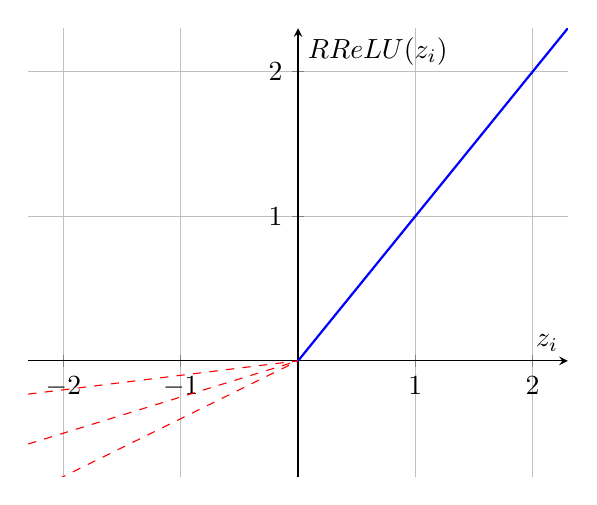
\begin{tikzpicture}
        \begin{axis}[
            xlabel={$z_i$},
            ylabel={$\text{RReLU}(z_i)$},
            xmin=-2.3, xmax=2.3,
            ymin=-0.8, ymax=2.3,
            axis lines=middle,
            grid=major,
            legend pos=north west,
            legend style={font=\tiny}
        ]
        \addplot[blue, thick, domain=0:2.3] {x};
        \addplot[red, dashed, domain=-2.3:0, samples=2] {0.1*x};
        \addplot[red, dashed, domain=-2.3:0, samples=2] {0.25*x};
        \addplot[red, dashed, domain=-2.3:0, samples=2] {0.4*x};
        \end{axis}
    \end{tikzpicture}
    \label{fig:rrelu}
\end{figure}

Se conhecemos com a RReLU se comporta podemos também calcular a sua derivada, a qual será de extrema utilidade durante a retropropagação, fazendo que os pesos e vieses do modelo sejam ajustados e com base nisso ele consiga aprender melhor o problema que está sendo analisado. Como a RReLU utiliza a mesma fórmula que funções como a Leaky ReLU e a PReLU, nós podemos apenas repetir a expressão de sua derivada novamente, a qual será dada pela equação \ref{eq:rrelu-derivada}. Note que mesmo compartilhando a mesma fórmula, o termo $\alpha$ possui significado distintos em cada uma dessas funções, neste caso, ele é um valor aleatório dado pela distribuição $U(l, u)$.

Com relação ao problema da descontinuidade no ponto zero, nós podemos apenas escolher para qual valor essa função irá retornar neste caso, assim, vamos considerar que quando a sua entrada for zero, ela irá retornar o segundo caso, em que é a própria constante $\alpha$

\begin{equacaodestaque}{Derivada Randomized Leaky ReLU (RReLU)}
    \frac{d}{dz_i} [RReLU](z_i) = \begin{cases}1, & \text{se } z_i > 0 \\ \alpha_i, & \text{se } z_i \leqslant  0 \end{cases}
    \label{eq:rrelu-derivada}
\end{equacaodestaque}

Esse detalhe da aleatoriedade da constante $\alpha$ afetou o desenho do gráfico da RReLU, e com isso, ele também afeta a plotagem de sua derivada. Como nós podemos ver na figura \ref{fig:rrelu-derivada}, existem um conjunto de retas em um intervalo, neste caso, estamos considerando a distribuição como sendo de $U(0.1, 0.3)$, mas para cada uma dessas distribuições, teremos um conjunto de retas diferentes e com isso gráficos distintos para cada um dos problemas.

\begin{figure}[h!]
    \centering
    \caption{Gráfico da Derivada da Função Randomized Leaky ReLU (RReLU) com $l=0.1, u=0.3$}
    \begin{tikzpicture}
        \begin{axis}[
            xlabel={$z_i$},
            ylabel={$\text{RReLU}'(z_i)$},
            xmin=-2.3, xmax=2.3,
            ymin=-0.2, ymax=1.2,
            axis lines=middle,
            grid=major,
            legend pos=north west,
            legend style={font=\scriptsize}
        ]
        % Define l e u para a distribuição uniforme U(l,u)
        \def\lVal{0.1}
        \def\uVal{0.3}

        % Plota a derivada para z > 0
        \addplot[red, thick, domain=0:2.1] {1};
        \addlegendentry{$f'(z_i) = 1$}

        % Plota a região hachurada para z < 0
        \addplot[
            pattern=north east lines, 
            pattern color=blue!50,
            draw=none
        ] coordinates {(-2.1, \lVal) (0, \lVal) (0, \uVal) (-2.1, \uVal)} -- cycle;
        \addlegendentry{$\alpha_i \sim U(l,u)$}

        % Marcadores na descontinuidade
        \addplot[blue, only marks, mark=o, mark size=1.5pt, forget plot] coordinates {(0,\lVal)};
        \addplot[blue, only marks, mark=o, mark size=1.5pt, forget plot] coordinates {(0,\uVal)};
        \addplot[red, only marks, mark=*, mark size=1.5pt, forget plot] coordinates {(0,1)};
        
        \end{axis}
    \end{tikzpicture}
    \label{fig:rrelu-derivada}
\end{figure}

Ainda no artigo, \textcite{XuRReLU} investigam a performance de diferentes funções retificadoras em uma rede neural convolucional, cuja arquitetura pode ser vista na tabela \ref{tab:nin_arquitetura}, para a classificação de imagens, os autores analisaram a ReLU tradicional, a Leaky ReLU, a Parametric ReLU e a Randomized Leaky ReLU. Para fazer a análise dos modelos, foram escolhidos os datasets CIFAR-10 e CIFAR-100, e o desempenho dessas funções nos respectivos datasets pode ser visto nas tabelas \ref{tab:ativacoes_cifar10} e \ref{tab:erro_ativacoes_cifar100}.

\begin{table}[ht]
    \caption{Estrutura da Rede "Network in Network" (NIN) para CIFAR-10/100}
    \label{tab:nin_arquitetura}
    \centering
    \begin{tabular}{ll}
        \toprule
        \textbf{Tamanho da Entrada} & \textbf{Camada / Operação} \\
        \midrule
        
        $32 \times 32$ & Conv 5x5, 192 canais \\
        $32 \times 32$ & Conv 1x1, 160 canais \\
        $32 \times 32$ & Conv 1x1, 96 canais \\
        $32 \times 32$ & Max Pooling 3x3, stride /2 \\
        \addlinespace % Adiciona espaço para separar os blocos
        
        $16 \times 16$ & Dropout, taxa 0.5 \\
        $16 \times 16$ & Conv 5x5, 192 canais \\
        $16 \times 16$ & Conv 1x1, 192 canais \\
        $16 \times 16$ & Conv 1x1, 192 canais \\
        $16 \times 16$ & Avg Pooling 3x3, stride /2 \\
        \addlinespace
        
        $8 \times 8$ & Dropout, taxa 0.5 \\
        $8 \times 8$ & Conv 3x3, 192 canais \\
        $8 \times 8$ & Conv 1x1, 192 canais \\
        $8 \times 8$ & Conv 1x1, 10 ou 100 canais\textsuperscript{a} \\
        $8 \times 8$ & Global Avg Pooling 8x8 \\
        \addlinespace
        
        10 ou 100 & Softmax \\
        
        \bottomrule
    \end{tabular}
    \vspace{2mm}
    
    \parbox{\linewidth}{\small
        \textit{Nota.} Descrição da arquitetura da rede convolucional "Network in Network" (NIN). A coluna "Tamanho da Entrada" indica a dimensão espacial dos mapas de características em cada estágio. A coluna "Camada / Operação" detalha a sequência de operações da rede.
        \textsuperscript{a}O número de canais na última camada convolucional corresponde ao número de classes do dataset (10 para CIFAR-10 ou 100 para CIFAR-100), funcionando como uma etapa de classificação antes do Global Average Pooling.
        Adaptado de "Empirical Evaluation of Rectified Activations in Convolutional Network", por B. Xu, N. Wang, T. Chen, \& M. Li, 2015, \textit{arXiv preprint arXiv:1505.00853}.
    }
\end{table}

Analisando a tabela \ref{tab:ativacoes_cifar10}, que mostra a taxa de erro das funções retificadoras na rede NIN para o dataset CIFAR-10, nós podemos notar que a Randomized Leaky ReLU foi a função que performou melhor, com um total de 11.19\% de erro nos casos de teste, enquanto a leaky ReLU com $a = 100$ obteve o pior resultado. Contudo, essa diferença de resultado é pequena, indicando que caso essas funções sejam muito mais complexas quando comparadas com a ReLU na hora de treinar o modelo, pode ser melhor optar por uma função mais "barata" mas com uma taxa de erro um pouco maior.

\begin{table}[ht]
    \caption{Taxa de Erro de Diferentes Funções de Ativação na Rede NIN para o CIFAR-10}
    \label{tab:ativacoes_cifar10}
    \centering
    \begin{tabular}{lcc}
        \toprule
        \textbf{Função de Ativação} & \textbf{Erro de Treino} & \textbf{Erro de Teste (\%)} \\
        \midrule
        
        ReLU                      & 0.00318 & 12.45 \\
        \addlinespace % Adiciona um espaço para agrupar as Leaky ReLUs
        Leaky ReLU ($a=100$)      & 0.00310 & 12.66 \\
        Leaky ReLU ($a=5.5$)      & 0.00362 & 11.20 \\
        \addlinespace
        PReLU                     & 0.00178 & 11.79 \\
        \addlinespace
        RReLU\textsuperscript{a}  & 0.00550 & \textbf{11.19} \\
        
        \bottomrule
    \end{tabular}
    \vspace{2mm}
    
    \parbox{\linewidth}{\small
        \textit{Nota.} Comparação da taxa de erro da rede "Network in Network" (NIN) treinada no conjunto de dados CIFAR-10 com diferentes funções de ativação retificadoras. Os valores de erro de teste são apresentados em porcentagem (\%). O valor em negrito indica o melhor resultado (menor erro de teste).
        \textsuperscript{a}Randomized Leaky ReLU (RReLU), onde o coeficiente de vazamento é amostrado de uma distribuição uniforme durante o treino. A fórmula na tabela original representa uma parametrização específica testada.
        Adaptado de "Empirical Evaluation of Rectified Activations in Convolutional Network", por B. Xu, N. Wang, T. Chen, \& M. Li, 2015, \textit{arXiv preprint arXiv:1505.00853}.
    }
\end{table}

Já ao analisarmos a tabela \ref{tab:erro_ativacoes_cifar100}, que nos mostra a taxa de erro dessas funções no dataset CIFAR-10, vemos que assim como no CIFAR-10, a RReLU foi a função que obteve melhor resultado, neste caso nós vemos uma diferença de 2.65 pontos percentuais, quando comparada com a ReLU tradicional. Outro ponto interessante a ser destacado ao analisar essa tabela é de que provavelmente a rede que utilizou a Parametric ReLU sofreu um sobreajuste (\textit{overfitting}) fazendo com que ela decorasse o dados de treino e com isso conseguisse uma taxa de erro consideravelmente menor, já quando ela foi apresentada para o conjunto de testes houve uma grande disparidade das taxas de erro.

\begin{table}[ht]
    \caption{Taxa de Erro de Funções de Ativação na Rede NIN para o CIFAR-100}
    \label{tab:erro_ativacoes_cifar100}
    \centering
    \begin{tabular}{lcc}
        \toprule
        \textbf{Função de Ativação} & \textbf{Erro de Treino (\%)} & \textbf{Erro de Teste (\%)} \\
        \midrule
        
        ReLU                      & 13.56 & 42.90 \\
        \addlinespace
        Leaky ReLU ($a=100$)      & 11.55 & 42.05 \\
        Leaky ReLU ($a=5.5$)      & 8.54  & 40.42 \\
        \addlinespace
        PReLU                     & \textbf{6.33}  & 41.63 \\
        \addlinespace
        RReLU\textsuperscript{a}  & 11.41 & \textbf{40.25} \\
        
        \bottomrule
    \end{tabular}
    \vspace{2mm}
    
    \parbox{\linewidth}{\small
        \textit{Nota.} Comparação da taxa de erro (\%) da rede "Network in Network" (NIN) treinada no conjunto de dados CIFAR-100. Os valores em negrito indicam o melhor resultado (menor erro) em cada coluna.
        \textsuperscript{a}Randomized Leaky ReLU (RReLU), onde o coeficiente de vazamento é amostrado de uma distribuição uniforme durante o treino.
        Adaptado de "Empirical Evaluation of Rectified Activations in Convolutional Network", por B. Xu, N. Wang, T. Chen, \& M. Li, 2015, \textit{arXiv preprint arXiv:1505.00853}.
    }
\end{table}

Ainda em \textit{Empirical Evaluation of Rectified Activations in Convolutional Network} \textcite{XuRReLU} explicam que a RReLU é uma função que ajuda a combater o sobreajuste (overfitting) do modelo, mas ainda devem ser feitos mais testes para descobrir como a aleatoriedade afeta os processos de treino e teste \parencite{XuRReLU}. Essa característica de ajudar a combater o sobreajuste é uma vantagem que a RReLU possui, permitindo com que modelos maiores e mais profundos possam ser criados e mesmo assim obtenham resultados significativos. Provavelmente, um dos motivos dela possuir essa função está no fato de que ela introduz uma maior aleatoriedade para o modelo, ajudando a impedir que ele decore os padrões, como em imagens dos conjuntos CIFAR-10 e CIFAR-100.

Considerando as fórmulas da RReLU, podemos construir o seu bloco de código \ref{lst:codigo-rrelu} que é capaz de implementar uma classe em python para atuar como a função Randomized Leaky ReLU.

\textbf{Implementação em Python}

\section{Em Busca da Suavidade: As Variantes Não Lineares}

Seguindo adiante, agora veremos um novo conjunto de variantes da ReLU tradicional, elas incluem funções que apresentam gráficos com curvas mais suaves, como é o caso da ELU, que faz uso de funções exponenciais para a sua composição e com isso consegue não só resolver o problema do neurônios agonizantes, mas também sendo uma função contínua em na origem e portanto derivável em todo o seu domínio.

Além disso, veremos uma variante da ELU, a Scaled Exponetial Linear Unit, uma função que é utilizada para construir redes capazes de se autonormalizarem, ademais veremos a Noisy ReLU, outra variante da ReLU, mas que dessa vez adiciona ruído em sua saída a fim de garantir uma melhor performance quando comparada com a sua função original.

\subsection{Exponential Linear Unit (ELU)}

Continuando com as alogias do vendedor de pipoca, o vendedor de pipoca que faz uso da ELU para as suas vendas trabalha de forma diferente. Ao invés de vender um punhado de pipoca de forma linear com base no dinheiro que o cliente tem quando ele não quer comprar o pacote inteiro por não possuir o valor total, ele adota uma curva exponencial como base, assim, clientes com valores muito próximos de R\$ 5,00 recebem uma quantia muito grande de pipoca, quase equivalente ao pacote total, enquanto aqueles que possuem valores pequenos irão receber um punhado pequeno de pipoca. Talvés seja uma forma de incentivar aqueles que quase tem o valor total para comprar uma pipoca, mas ainda sim garantir a clientela dos que possuem pouco dinheiro e aumentando o seu lucro como vendendor.

A ELU ou Exponential Linear Unit foi introduzida no artigo \textit{Fast and Accurate Deep Networks Leaning By Exponential Linear Units (ELUs)}, sendo uma variação que acelera o aprendizado de uma rede neural densa e apresentando uma maior acurácia em problemas de classificação \parencite{ELUArticle}. Um dos testes realizados pelos autores para analisar o desempenho na ELU, foi na criação de uma CNN com 18 camadas convolucionais para fazer a classifição dos datasets CIFAR-10 e CIFAR-100, para isso, outras técnicas foram utilizas em conjunto como o decaimento do peso L2 e reduções das taxas de aprendizado \parencite{ELUArticle}.

Com base nessa CNN e seus experimentos, é possível ver os resultados na tabela \ref{tab:elu_cifar_comparativo}, em que \textcite{ELUArticle} comparam a ELU com outras redes no mesmo problema, como a AlexNet que vimos anterioremente na explicação do surgimento da ReLU. Ao analisarmos esses resultados, vemos que a ELU obteve um desempenho excelente no dataset CIFAR-100, com uma diferença de 21.52 pontos percentuais quando comparada com a AlexNet, que ficou em último lugar. Já quando analisamos o seu desempenho para um problema de classificação mais simples, como o CIFAR-10, ela ficou em segundo lugar, estando atrás apenas da Fract. Max-POoling, mas ainda sim, apresentando uma diferença considerável de 2.05 pontos percentuais a mais de erro. 

\begin{table}[ht]
    \caption{Comparativo da Taxa de Erro de Redes Neurais nos Datasets CIFAR}
    \label{tab:elu_cifar_comparativo}
    \centering
    \begin{tabular}{lccc}
        \toprule
        \textbf{Arquitetura da Rede} & \textbf{CIFAR-10 Erro (\%)} & \textbf{CIFAR-100 Erro (\%)} & \textbf{Augmentation} \\
        \midrule
        
        AlexNet              & 18.04          & 45.80          &                \\ 
        \addlinespace
        DSN                  & 7.97           & 34.57          & v              \\
        NiN                  & 8.81           & 35.68          & v              \\
        Maxout               & 9.38           & 38.57          & v              \\
        All-CNN              & 7.25           & 33.71          & v              \\
        Highway Network      & 7.60           & 32.24          & v              \\
        Fract. Max-Pooling   & \textbf{4.50}  & 27.62          & v              \\
        ELU-Network          & 6.55           & \textbf{24.28} & v              \\
        
        \bottomrule
    \end{tabular}
    \vspace{2mm}
    
    \parbox{\linewidth}{\small
        \textit{Nota.} Comparação da taxa de erro de classificação (\%) no conjunto de teste para diversas arquiteturas de redes neurais convolucionais (CNNs). Os valores em negrito indicam o melhor resultado em cada dataset.
        A coluna "Augmentation" indica se foram utilizadas técnicas de aumento de dados (data augmentation) durante o treinamento, marcado com "v".
        Adaptado de "Fast and Accurate Deep Network Learning by Exponential Linear Units (ELUs)", por D. Clevert, T. Unterthiner, \& S. Hochreiter, 2015, \textit{arXiv preprint arXiv:1511.07289}.
    }
\end{table}

Isso nos indica que a ELU é uma excelente opção para problemas de classificação, especialmente se tivermos um grande número de classes a ser analisados. Contudo, uma rede neural convolucional que apresenta 18 camadas de convolução pode ser um tanto quanto custosa para ser processada por um computador, assim, faz se necessário o uso de unidades de GPUs para o processamento de uma rede como essa, para que mesmo sendo pesada para ser processada, os resultados possam sair um pouco mais rápidos. Em uma das seções a frente, será possível comparar o desempenho das funções retificadoras as quais estamos vendo nesse texto, e a partir desses comparativos, veremos que talvez não seja uma opção interessante utilizar funções que fazem uso de exponenciais em suas fórmulas para resolver problemas de classificação mais simples, como o caso do dataset CIFAR-10.

Agora que entendendo que a ELU pode ser uma boa alternativa para problemas de classifacação de múltiplas classes, podemos conhecer como ela é escrita e como se comporta graficamente. A Exponential Linear Unit pode é descrita utilizando a expressão \ref{EquacaoELU}. Note que temos uma grande diferença dela quando comparamos com a ReLU, a Exponential Linear Unit faz uso de funções exponenciais, algo que é computacionalmente mais pesado para um computador quando comparado com apenas cálculos simples como uma função identidade, podemos esperar que ela será mais lenta quando comparamos com a ReLU, mas para ter certeza precisaremos fazer comprativos, os quais serão vistos futuramente.

\begin{equacaodestaque}{Exponential Linear Unit (ELU)}
    \text{ELU}(z_i) = \begin{cases}z_i, & \text{se } z_i \ge 0 \\ \alpha \cdot (e^{z_i} - 1), & \text{se } z_i < 0\end{cases}
    \label{eq:elu}
\end{equacaodestaque}

Conhecendo como é a fórmula da ELU, podemos também plotar o seu gráfico, o qual está presente na figura \ref{fig:GraficoELU}. Ao analisarmos, vemos uma diferença notável quando o comparamos com as funções vistas anterioemente, a ELU não apresenta um bico no ponto de origem, ela é uma função bem mais suave. Além disso, vemos que ela segue o mesmo padrão das outras funções: ela retorna a função identidade nos casos em que a entrada é maior que zero, assim como as outras variantes, mas quando analisamos a os casos em que a entrada é negativa, vemos que ela utiliza uma funcão exponencial, o que garante a suavidade vista no gráfico. Podemos notar também que ela possui valores negativos, assim como as variantes com vazamento, indicando que ela também pode ser capaz de lidar com o problema do neurônios agonizantes causado pela ReLU tradicional e que vem sendo mitigado com outras variantes como a Leaky ReLU.

\begin{figure}[h!]
    \centering
    \caption{Gráfico da Função Exponential Linear Unit (ELU) com $\alpha=1$}
    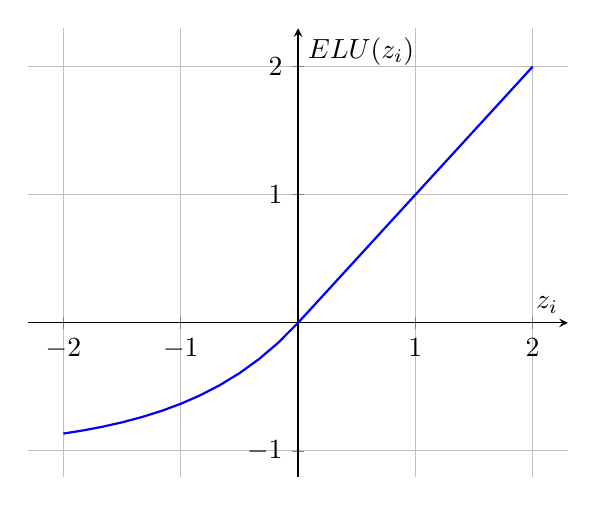
\begin{tikzpicture}
        \begin{axis}[
            xlabel={$z_i$},
            ylabel={$\text{ELU}(z_i)$},
            xmin=-2.3, xmax=2.3,
            ymin=-1.2, ymax=2.3,
            axis lines=middle,
            grid=major,
        ]
        % Define alpha para o gráfico. O valor comum para ELU é 1.
        \def\alphaVal{1} 
        \addplot[blue, thick, domain=-2:2] {x >= 0 ? x : \alphaVal*(exp(x) - 1)};
        \end{axis}
    \end{tikzpicture}
    \label{fig:elu}
\end{figure}

Já que sabemos a sua fórmula e o seu gráfico, podemos também calcular a sua derivada, a qual será útil na retropropagação do modelo. Para isso, seguimos a mesma estratégia vista até agora, derivamos a função em cada um dos casos, gerando assim a sua derivada. Nos cenários em que a entrada é positiva, a derivada será sempre 1, pois quando derivamos a expressão $x$, ela nos irá retornar 1. Já quando temos o cenário negativo, teremos como resultado da derivação da expressão $alpha \cdot (e^{z_i} - 1)$ o termo $alpha \cdot e^{z_i}$. Um ponto a ser destacado é de que a ELU é contínua na origem, assim, não temos que nos preocupar em escolher um valor da derivada quando o seu valor de entrada for zero. Assim, temos como resultado final a expressão \ref{eq:DerivadaELU}

Para calcularmos sua derivada, basta derivamos as duas expressões da equação \ref{eq:EquacaoELU} encontrando então a função \ref{eq:DerivadaELU}.

\begin{equacaodestaque}{Derivada Exponential Linear Unit (ELU)}
    \frac{d}{dz_i} [ELU](z_i) = \begin{cases}1, & \text{se } z_i > 0 \\ \alpha \cdot e^{z_i}, & \text{se } z_i \le 0 \end{cases}
    \label{eq:elu-derivada}
\end{equacaodestaque}

Sabendo a sua derivada, podemos também plotar o seu gráfico, para isso, temos a figura \ref{fig:GraficoELUDerivada}. Note que ele é composto de duas partes diferentes, sendo a primeira delas, para os casos em que a entrada é negativa, a função constante em um, e para os casos em que a entrada é negativa, nós temos uma curva exponencial. Podemos notar também que a sua derivada irá sempre retornar valores positivos quando é calcula para qualquer ponto do seu domínio.

\begin{figure}[h!]
    \centering
    \caption{Gráfico da Derivada da Função Exponential Linear Unit (ELU) com $\alpha=1$}
    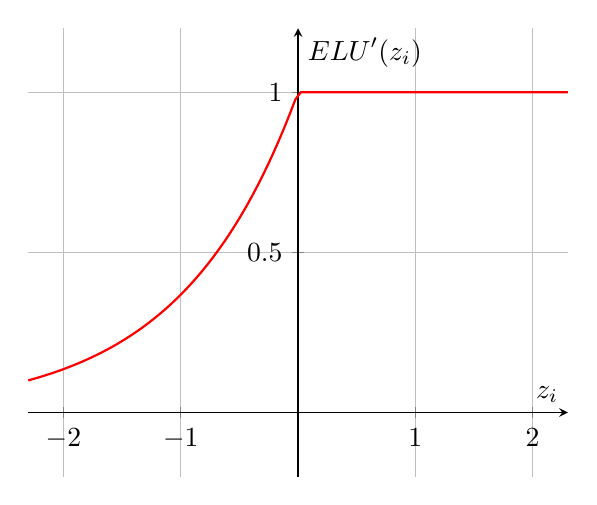
\begin{tikzpicture}
        \begin{axis}[
            xlabel={$z_i$},
            ylabel={$\text{ELU}'(z_i)$},
            xmin=-2.3, xmax=2.3,
            ymin=-0.2, ymax=1.2,
            axis lines=middle,
            grid=major
        ]
        % Define alpha para o gráfico
        \def\alphaVal{1} 

        % Plota a derivada usando uma única expressão condicional
        \addplot[red, thick, domain=-2.3:2.3, samples=100] {x > 0 ? 1 : \alphaVal*exp(x)};
        
        \end{axis}
    \end{tikzpicture}
    \label{fig:elu-derivada}
\end{figure}

Por fim, cabe destacar algumas afirmações realizadas pelos autores ainda em \textit{Fast and Accurate Deep Networks Leaning By Exponential Linear Units (ELUs)}, segundo \textcite{ELUArticle}, quando nós comparamos a ELU com funções como a ReLU tradicional e Leaky ReLU, nós podemos notar um melhor e mais rápido aprendizado, além de que a Exponetial Linear Unit é capaz de garantir uma melhor generalização quando passa a ser utilizada em redes com mais de cinco camadas. Outro ponto destacado pelos autores, está no fato da ELU garantir noise rebust deactivation states, algo que mesmo com a Leaky ReLU e Parametric ReLU possuindo valores negativos, não são capazes de garantir ao serem utilizadas para construir uma rede neural.

Mesmo apresentando um grande salto, quando comparada com a ReLU tradicional, a ELU também pode ser modificada para atender outros casos. Para isso, ela também tem variações, sendo uma delas a SELU, a qual adiciona a ELU um termo $\lambda$ para garantir uma autonormalização da rede que está sendo criada. Nós veremos essa função em seguida.

\textbf{Implementação em Python}

\subsection{Scaled Exponential Linear Unit (SELU)}

A próxima função que iremos conhecer é uma variante da ELU, a Scaled Exponential Linear Unit, ou SELU. Ela se distingue da ELU tradicional pelo fato de que ela é capaz de implemtar propriedades auto-normalizadoras em uma rede que faz uso dessa função, como explicam os autores no aritofo de sua introdução \textit{Self-Normalizing Neural Networks} \parencite{SELUArticle}.

No texto, \textcite{SELUArticle}, comparam as redes neurais criadas por eles, as quais são chamadas de Self-Normalizing Neural Networks (SNN), com outras redes feedforward, como MSRAinit (uma FNN que não possui técnicas de normalização, com funções de ativação ReLU, e que faz uso do Microsoft weight initialization), a BatchNorm (uma FNN com normalização em lote), a LayerNorm (uma FNN com normalização nas camadas), a WightNorm (uma FNN com normalização nos pesos), a Highway e também com redes residuais ResNet. Para comparar essas redes, os autores escolhem 121 datasets do UCI, em que são apresentadas áreas de aplicação diversas como física e biologia, nesses dadatasets o seus tamanhos podem variar de 10 até 130.000 pontos de dados com o número de features variando de 4 a 250, na tabela \ref{tab:comparativo-selu}, é possível ver o ranking médio entre as SNNs e as outras diferentes arquiteturas em 75 tarefas de classificação.

\begin{table}[ht]
    \caption{Comparativo do Rank Médio entre SNNs e Outras Arquiteturas de Redes Neurais}
    \label{tab:comparativo-selu}
    \centering
    \begin{tabular}{llcc}
        \toprule
        \textbf{Grupo do Método} & \textbf{Método} & \textbf{Rank Médio} & \textbf{Valor-p} \\
        \midrule
        
        SNN & SNN & 9.6 & $3.8 \times 10^{-1}$ \\
        MSRAinit & MSRAinit & 11.0 & $4.0 \times 10^{-2}$ \\
        LayerNorm & LayerNorm & 11.3 & $7.2 \times 10^{-2}$ \\
        Highway & Highway & 11.5 & $8.9 \times 10^{-3}$ \\
        ResNet & ResNet & 12.3 & $3.5 \times 10^{-3}$ \\
        BatchNorm & BatchNorm & 12.6 & $4.9 \times 10^{-4}$ \\
        WeightNorm & WeightNorm & 13.0 & $8.3 \times 10^{-5}$ \\

        \bottomrule
    \end{tabular}
    \vspace{2mm}
    
    \parbox{\linewidth}{\small
        \textit{Nota.} Comparação do rank médio de diferentes arquiteturas de redes neurais em 75 tarefas de classificação do repositório UCI. O "Rank Médio" é a média das classificações de acurácia entre as tarefas. O "Valor-p" corresponde ao teste de Wilcoxon pareado para avaliar se a diferença para o método de melhor desempenho é significativa.
        Adaptado de "Self-Normalizing Neural Networks", por G. Klambauer, T. Unterthiner, A. Mayr, \& S. Hochreiter, 2017, \textit{arXiv preprint arXiv:1706.02515}.
    }
\end{table}

Para analisar essa tabela, podemos primeiro olhar o ranking médio de cada uma desses modelos, que é dado pela média de como esses modelos performaram nos diferentes datasets, considerando isso, nós notamos que as redes que fazem uso da SELU em sua composição, as SNNs, são as melhores, por uma diferença de 1.4 pontos quando comparadas com o segundo colocado, isso nos indica que a SELU pode ser uma ótima alternativa quando ainda não se sabe exatamente qual será o conjunto de dados que será trabalhado, se ele será de conceitos como física ou geologia, assim, elas garantem uma maior versatilidade para encarar diversos problemas. Além disso, se olharmos também o seu p-value, que vem de um teste de Wilcoxon pareado para verificar se a diferença em relação ao melhor colocado é signifitiva, vemos que as SNNs continuam se destacando, com o p-value mais alto, indicando que existe uma diferença que não é estatisticamente significativa quando ela é comparada com o modelo SVM, nos mostrando que podemos considerar as SNNs como se tivessem empatadas com o campeão.

O interessante dessa comparação é olharmos ela considerando aquelas redes que fazem uso de técnicas de normalização para conseguir uma maior desempenho, como a BatchNorm e a LayerNorm, cada uma delas utiliza uma técnica de normalização diferente de forma a garantir que que problemas como os gradientes explosivos e fuga do gradiente não ocorra com tanta frequência e com isso permitindo um melhor convergência do modelo que está sendo treinado. Se olharmos por essa ótica, podemos chegar a conclusão que criar uma rede neural utilizando a SELU não só ura garantir uma maior versatilidade para a resolução de problemas, como também não teremos que nos preocupar em aplicar técnicas de normalização ao construir essa rede.

Agora que temos uma noção maior de como a SELU pode ser uma opção interessante para criar uma RNA, podemos conhecer como ela funciona de fato. Para isso, os autores apresentam a fórmula \ref{eq:EquacaoSELU} para calcular essa função, em que o termo $\lambda$ é uma constante que será maior que 1 \parencite{SELUArticle}. Note que essa fórmula é bem parecida com a da Exponential Linear Unit, a única diferença é que ela estará sendo multiplicada pela constante $\lambda$, assim podemos escrever também que $\text{SELU}(z_i) = \lambda \text{ELU}(z_i)$.

\begin{equacaodestaque}{Scaled Exponential Linear Unit (ELU)}
    \text{SELU}(z_i) = \lambda \begin{cases}z_i, & \text{se } z_i > 0 \\ \alpha \cdot (e^{z_i} - 1), & \text{se } z_i \le 0\end{cases}
    \label{eq:selu}
\end{equacaodestaque}

Conhendo sua equação, podemos também plotar o seu gráfico, o qual está presente na figura \ref{fig:GraficoSELU}, neste caso, estamos considerando que as constantes $\alpha$ e $\lambda$ são dados por 1.7 e 1.05 respectivamente. Podemos notar que é um gráfico que lembra bastante a Leaky ReLU, mas que neste caso, quando a função recebe valores negativos, ela não estará mais assumindo o comportamento de uma reta, e sim o de uma curva exponencial, já para os cenários em que a entrada é postiva os resultados serão próximos os de uma função identidade, mas com uma reta um pouco mais inclinada. 

Pelo fato da SELU ter um comportamento que também retorna valores para a saída quando a sua entrada é negativa, ela consegue combater o problema dos Dying ReLUs, causado pela ReLU, além de que também não é uma função saturante, como a sigmoide, o que também ajuda a resolver o problema da fuga dos gradientes. Mas, por não ser uma função saturante, e pelo fato de que sua saída vai para valores infinitos conforme os valores de sua entrada aumentam, ela está sujeita ao problema da explosão de gradientes.

\begin{figure}[h!]
    \centering
    \caption{Gráfico da Função Scaled Exponential Linear Unit (SELU) com $\alpha \approx 1.67 e \lambda \approx 1.05$}
    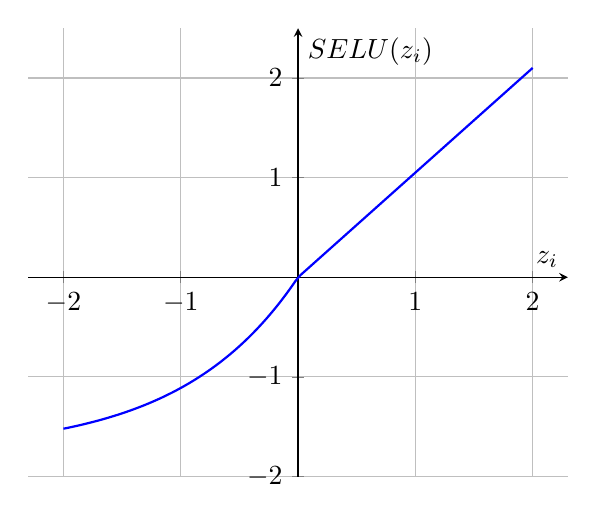
\begin{tikzpicture}
        \begin{axis}[
            xlabel={$z_i$},
            ylabel={$\text{SELU}(z_i)$},
            xmin=-2.3, xmax=2.3,
            ymin=-2, ymax=2.5,
            axis lines=middle,
            grid=major,
        ]
        % Define as constantes da SELU para o gráfico
        \def\alphaVal{1.67326}
        \def\lambdaVal{1.0507}
        \addplot[blue, thick, domain=-2:2, samples=100] {x > 0 ? \lambdaVal*x : \lambdaVal*\alphaVal*(exp(x) - 1)};
        \end{axis}
    \end{tikzpicture}
    \label{fig:selu}
\end{figure}

Considerando agora que sabemos como é a equação da SELU e qual é o seu comportamento no gráfico, podemos também calcular a sua derivada para utilizarmos na retroproapagação do gradiente, para isso, devemos derivar a expressão \ref{eq:EquacaoSELU}, considerando os dois cenários, em que a sua entrada será positiva e quando sua entrada for negativa ou zero. Um ponto que nos ajuda bastante ao calcular a derivada da SELU está no fato dela ser composta pela função ELU multiplicada por uma constante, se utilizarmos regras de derivação para esse cenário, precisaremos apenas derivar a ELU e depois adicionar a constante $\lambda$ multiplicando-a. Como nós já calculamos a derivada da ELU, podemos ver então a derivada da Scaled Exponential Linear Unit na equação \ref{eq:DerivadaSELU}.

\begin{equacaodestaque}{Derivada Scaled Exponential Linear Unit (ELU)}
    \frac{d}{dz_i} [SELU](z_i) = \lambda \begin{cases}1, & \text{se } z_i > 0 \\ \alpha \cdot e^{z_i}, & \text{se } z_i \le 0\end{cases}
    \label{eq:selu-derivada}
\end{equacaodestaque}

Se sabemos a sua derivada, podemos também plotar o seu gráfico, para isso, temos a representação na figura \ref{fig:GraficoSELUDerivada}. Note, que o gráfico da derivada da SELU também possui grandes similaridades com a ELU original mas também com as outras retificadoras, pois também pode ser dividido em duas partes principais. A primeira parte, para os casos em que a entrada é negativa segue o comportamento de uma curva exponencial, enquanto a segunda parte é semelhante a uma reta constante com inclinação zero. 

Um ponto interessante dessa reta da segunda parte é que ela retorna justamente um valor bem próximo de um, assim como nas retificadoras, isso trás como benefício uma menor chance para ocorrer casos de fuga de gradiente, pois ele não estará sendo constantemente sendo multiplicado por valores pequenos e com isso reduzindo o seu valor. Mas, por outro lado, isso também acaba colaborando para que gradientes explosivos possam ocorrer.

\begin{figure}[h!]
    \centering
    \caption{Gráfico da Derivada da Função Scaled Exponential Linear Unit (SELU) com $\alpha \approx 1.67, \lambda \approx 1.05$}
    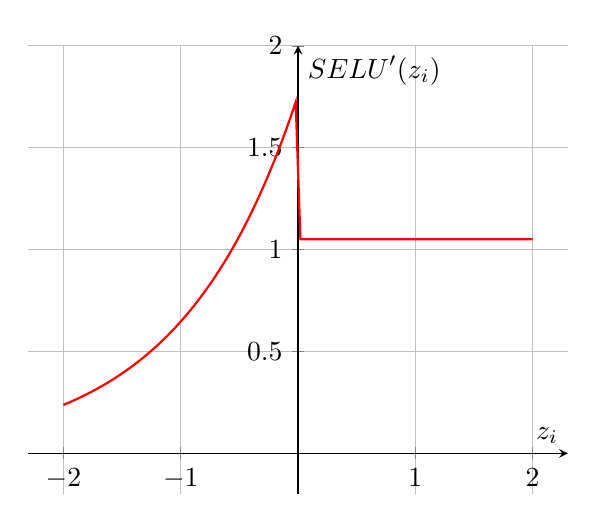
\begin{tikzpicture}
        \begin{axis}[
            xlabel={$z_i$},
            ylabel={$\text{SELU}'(z_i)$},
            xmin=-2.3, xmax=2.3,
            ymin=-0.2, ymax=2.0, % Ajustado para lambda > 1
            axis lines=middle,
            grid=major
        ]
        % Define as constantes da SELU para o gráfico
        \def\alphaVal{1.67326}
        \def\lambdaVal{1.0507}

        \addplot[red, thick, domain=-2:2, samples=100] {x > 0 ? \lambdaVal*1 : \lambdaVal*\alphaVal*exp(x)};
        \end{axis}
    \end{tikzpicture}
    \label{fig:selu-derivada}
\end{figure}

Voltando para o seu texto de introdução, os autores destacam propriedades importantes dessa nova função de atiavção criada, como o fato de que de que elas possbilitam a criação de redes neurais mais profundas além de serem capazes de aplicar fortes esquemas de regularização \parencite{SELUArticle}. Por favorecer a criação de RNAs mais profundas, como consequência, a SELU se torna uma excelente alternativa para ser utilizada em problemas complexos, que possuem muitas características e por essa razação necessitam de que mais camadas sejam construídas a fim de garantir um melhor processamento e aprendizado dos dados e com base nisso, alcançar métricas maiores, como uma maior acurácia indicando uma gerenalização maior e também uma perda menor, indicando que o gradiente conseguiu uma convergência melhor.

\textbf{Implementação em Python}

\subsection{Noisy ReLU}

Seguindo adiante, a última variante da ReLU que iremos ver nessa seção das variantes suaves, é a Noisy ReLU, também conhecida como NReLU. Um dos trabalhos que explora as característica dessa função e como ela pode ser aplicada em uma RNA é o \text{Rectified Linear Units Improve Restricted Boltzmann Machines} dos autores \textcite{Nair2010}. Nesse texto, os autores comparam o desenpenho dessa função com a função binária, dada pela equação \ref{eq: equacao-binary}, que era a opção mais comum para ser utilizada na construção de máquinas restritas de Boltzmann.

\begin{equation}
    f(z_i) = \begin{cases} 
    1 & \text{se } z_i \ge \theta \\ 
    0 & \text{se } z_i < \theta 
    \end{cases}
    \label{eq: equacao-binary}
\end{equation}

Para entendermos como a comparação dessas funções ocorreu, é interessante primeiro conhecer o conceito das máquinas restritas de boltzmann.

\begin{quote}
    \textit{As Máquinas de Boltzmann Restritas (RBMs) têm sido usadas como modelos generativos de muitos tipos diferentes de dados, incluindo imagens rotuladas ou não rotuladas, sequências de coeficientes mel-cepstrais que representam a fala, sacos de palavras que representam documentos e classificações de usuários de filmes. Em sua forma condicional, elas podem ser usadas para modelar sequências temporais de alta dimensão, como dados de vídeo ou captura de movimento. Seu uso mais importante é como módulos de aprendizagem que são compostos para formar redes de crenças profundas.}

\hfill \textemdash (Nair \& Hinton, 2010, p. 1, tradução nossa)
\end{quote}

No trabalho, \textcite{Nair2010} exploram o desempenho dessas duas funções utilizando o dataset NORB, que é um dataset para o reconhecimento de objetos 3D sintéticos que contém cinco classes: humanos, animais, carros, aviões e caminhões. No texto, os autores utilização a vrsão Jittered-Cluttered NORB, uma variante que tem imagens estereoscópicas em tons de cinza com fundo desorganizado e um objeto central que é aleatoriamente instável em posição, tamanho, intensidade de pixels \parencite{Nair2010}. O desempenho dessas funções nesse dataset pode ser visto pelas tabelas \ref{tab:norb_error_rate} e \ref{tab:nrelu_norb_comparativo}.

A tabela \ref{tab:norb_error_rate}, nos mostra a taxa de erro dos diferentes modelos no dataset, para isso, são construídos modelos com 4000 unidades ocultas treinados com imagens de dimensões 32x32x2. Podemos notar ao analisar a tabela que é nítido que os modelos que são pré-treinados utilizando máquinas de Boltzmann restritas apresentam um melhor desempenho de forma geral, da mesma forma que a NReLU oferece uma perda menor quando comparada com a função binária em ambos os casos: pré-treinado ou não. 

Mas, podemos fazer uma comparação ainda mais interessante, o modelo que faz uso da Noisy ReLU que não foi pré-treinado apresenta um resultado com uma diferença de 0.9 pontos quando comparado com o modelo treinado que faz uso da função binária. Isso é interessante porque nos indica que podemos conseguir um resultado muito melhor utilizando a Noisy ReLU mediante a função binária mesmo quando não tivermos condições de pré-treinar uma rede.

\begin{table}[ht]
    \caption{Taxa de Erro de Classificadores no Dataset NORB Jittered-Cluttered}
    \label{tab:norb_error_rate}
    \centering
    \begin{tabular}{lcc}
        \toprule
        \textbf{Pré-treinado?} & \textbf{NReLU (\%)} & \textbf{Binary (\%)} \\
        \midrule
        
        Não & 17.8 & 23.0 \\
        Sim & \textbf{16.5} & \textbf{18.7} \\
        
        \bottomrule
    \end{tabular}
    \vspace{2mm}
    
    \parbox{\linewidth}{\small
        \textit{Nota.} Taxas de erro no conjunto de teste para classificadores com 4000 unidades ocultas. Os valores em negrito indicam a menor taxa de erro (melhor resultado) em cada coluna. Os modelos foram treinados com imagens de 32x32x2 do dataset NORB Jittered-Cluttered. A coluna "NReLU" refere-se a unidades de ativação ReLU com ruído (Noisy ReLU), enquanto "Binary" refere-se a unidades binárias tradicionais. A coluna "Pré-treinado?" indica se o modelo utilizou uma Máquina de Boltzmann Restrita para pré-treinamento.
        Adaptado de "Rectified Linear Units Improve Restricted Boltzmann Machines", por V. Nair \& G. E. Hinton, 2010, \textit{Proceedings of the 27th International Conference on Machine Learning (ICML-10)}.
    }
\end{table}

Seguindo adiante, na tabela \ref{tab:nrelu_norb_comparativo} tembém é possível analisar as taxas de erro dos classicadores, mas, neste caso, eles possuem duas camadas ao invés de somente uma como mostrado da comparação da tabela \ref{tab:norb_error_rate}, assim a primeira camada é composta de 4000 unidades ocultas (assim como no primeiro caso), enquanto a segunda camada possui 2000 unidades ocultas. 

Com base essa tabela nós podemos notar que o desempenho dos modelos que fazem uso da Noisy ReLU melhorou tanto nos casos em que as camadas não foram pré-treinadas, quanto nos casos em que uma ou ambas foram, quando se compara com os resultados da tabela \ref{tab:norb_error_rate}. Um ponto interessante disso é que no caso em que somente uma das camadas foi pré-treinada no modelo que usa a NReLU o seu resultado foi igual ao do primeiro caso onde existia somente uma camada, o que pode nos indicar que talvez não seja vantajoso adicionar mais camadas em uma rede caso não estejamos dispostos a pré-treiná-las. Note também que esse cenário com a unidade binária foi ainda pior, nos mostrando que não temos um grande ganho em adicionar mais camadas em uma rede que faz uso dessa função.

Esse resultado prová-se ainda mais nítido quando vemos o caso em que ambas as camadas foram pré-treinadas, na unidade binária não houve nenhuma diminuição na sua perda, ela inclusive é pior que a do modelo que faz uso de apenas uma camada. Já quando observamos a Noisy ReLU e seus resultados, vemos um cenário bem diferente, os modelos que fazem uso dela apresentam um desempenho melhor quando são adicionadas mais camadas na rede, fazendo com que a perda da rede diminua, indicando que essa função permite a criação de redes mais profundas e com isso, desempenhos melhores possam ser alcançados.

\begin{table}[ht]
    \caption{Taxas de Erro de Classificadores no Dataset Jittered-Cluttered NORB}
    \label{tab:nrelu_norb_comparativo}
    \centering
    \begin{tabular}{llcc}
        \toprule
        \multicolumn{2}{c}{\textbf{Camadas Pré-treinadas}} & \multicolumn{2}{c}{\textbf{Taxa de Erro de Teste (\%)}} \\
        \cmidrule(r){1-2} \cmidrule(r){3-4} % Linhas parciais para agrupar colunas
        \textbf{Camada 1} & \textbf{Camada 2} & \textbf{NReLU} & \textbf{Binary} \\
        \midrule
        
        Não & Não & 17.6 & 23.6 \\
        Sim & Não & 16.5 & \textbf{18.8} \\
        Sim & Sim & \textbf{15.2} & \textbf{18.8} \\
        
        \bottomrule
    \end{tabular}
    \vspace{2mm}
    
    \parbox{\linewidth}{\small
        \textit{Nota.} Taxas de erro (\%) de teste para classificadores com duas camadas ocultas (4000 unidades na primeira, 2000 na segunda), treinados em imagens do dataset Jittered-Cluttered NORB de 32x32x2. A tabela compara modelos com unidades retificadoras ruidosas (NReLU) e unidades binárias tradicionais (Binary), avaliando o impacto do pré-treinamento de cada camada. Os valores em negrito indicam os melhores resultados para cada tipo de unidade.
        Adaptado de "Rectified Linear Units Improve Restricted Boltzmann Machines", por V. Nair \& G. E. Hinton, 2010, \textit{Proceedings of the 27th International Conference on Machine Learning (ICML-10)}, pp. 807-814.
    }
\end{table}

Esse tópico de permitir a criação de redes mais profundas, que aconteceu justamente ao optar por funções retificadoras como a ReLU e a Noisy ReLU ao invés de funções sigmoide, está intrinsicamente relacionado ao problema da fuga do gradiente. Em redes que faziam uso de funções sigmoide, os programadores e pesquisadores estavam constantemente correndo o risco de que ao adicionar mais camadas a fim de que essa rede pudesse alcançar melhores métricas, o problema da fuga do gradiente viesse a tona. Isso acontece, porque ao adicionar mais camadas, existe uma maior chance de que esse vetor seja mais uma vez multiplicado por valores pequenos e com isso diminuísse o seu valor.

Sabendo de como a NReLU surgiu e sua importância para permitir a criação de redes mais profundas, podemos conhecer a sua fórmula e entender como ela funciona na prática. No texto, \textcite{Nair2010}, apresentam a NReLU como sendo dada pela equação $\max{0, z_i + \mathcal{N}(0, \sigma(z_i))}$, em que $\mathcal{N}(0, V)$ representa o ruído Gaussiano (Gaussian noise em inglês), com méida zero e vairância dada por $V$. Como neste texto estamos dando maior enfoque em uma notação com condicionais para as funções retificadoras, também podemos expressar a Noisy ReLU com a equação \ref{eq: EquacaoNReLU}.

\begin{equation}
    \text{NReLU}(z_i) = \begin{cases} 
    0 & \text{se } z_i \le 0 \\ 
    z_i + \mathcal{N} (0, \sigma(z_i)) & \text{se } z_i > 0 
    \end{cases}
    \label{eq: EquacaoNReLU}
\end{equation}

Antes de seguir em frente, é útil entende primeiro o que é ruído gaussiano, e para isso, precisamos entender antes a distribuição gaussiana. Segundo \textcite{DeepLearningBook}, a distribuição gaussiana é a distribuição mais utilizada para números reais, ela também é conhecida também por ser chamada de distribuição normal, ela é dada pela equação \ref{eq: DistribuicaoGaussiana}.

\begin{equation}
    \mathcal{N}(x; \mu, \sigma^2) = \sqrt{\frac{1}{2\pi\sigma^2}} \exp\left( -\frac{1}{2\sigma^2}(x - \mu)^2 \right)
    \label{eq: DistribuicaoGaussiana}
\end{equation}

Nessa equação, os dois parâmetros $\mu \in \mathbb{R}$ e $\sigma (0, \infty)$ controlam como a distribuição normal funciona; o termo $\mu$ é responsável por dar as coordenadas para o pico do centro, que é também a média da distribuição $\mathbb{E}[x] = \mu$, já o desvio padrão é dado por $\sigma$, equanto a variância é denotada por $\sigma^2$ \parencite{DeepLearningBook}. Para chegarmos no ruído gaussiano, precisamos então adicionar como parâmetros da equação da distribução gaussiana (equação \ref{eq: DistribuicaoGaussiana}) os termos que são dados pela equação \ref{eq: EquacaoNReLU}. 

A distribuição normal, com os parâmetros $\mu = 0$ e $\sigma=1$, é responsável por nos dar um gráfico em formato de sino, como é mostrado na figura \ref{fig:GraficoDistNormalPadrao}. Esse gráfico indica quais são os casos que possuem uma maior probabilidade de acontecer, os casos que estão no centro, onde, $p(x)$ possuem uma maior probabilidade de acontecer, já conforme eles se distânciam desse centro essa propabilidade diminui.

\begin{figure}[htbp]
    \centering
    \caption{Gráfico da Distribuição Gaussiana (ou Normal) para o caso padrão, com média 0 ($\mu = 0$) e desvio padrão 1 ($\sigma = 1$).}
    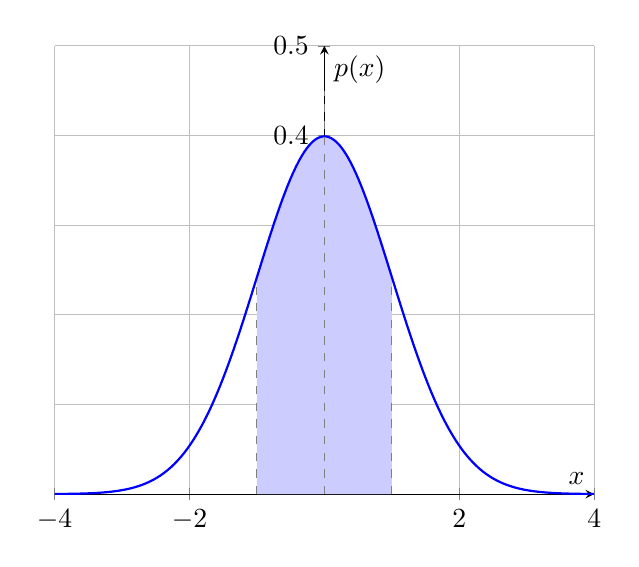
\begin{tikzpicture}
        \begin{axis}[
            xlabel={$x$},
            ylabel={$p(x)$}, % p(x) é a densidade de probabilidade
            xmin=-4, xmax=4,
            ymin=0, ymax=0.5,
            axis lines=middle,
            grid=major,
            samples=200, % Aumenta o número de pontos para uma curva mais suave
            domain=-4:4,
        ]
        
        % Declara a função da distribuição normal para facilitar o uso
        \def\normaldist#1#2{1/(#2*sqrt(2*pi))*exp(-((x-#1)^2)/(2*#2^2))}
        
        % Adiciona a área sombreada para +/- 1 desvio padrão
        \addplot[fill=blue!20, draw=none, domain=-1:1] {\normaldist{0}{1}} \closedcycle;

        % Plota a curva da distribuição normal padrão (mu=0, sigma=1)
        \addplot[blue, thick] {\normaldist{0}{1}};

        % Adiciona linhas verticais para marcar a média e os desvios padrão
        \draw[dashed, gray] (axis cs:0, 0) -- (axis cs:0, 0.45);
        \draw[dashed, gray] (axis cs:1, 0) -- (axis cs:1, 0.24);
        \draw[dashed, gray] (axis cs:-1, 0) -- (axis cs:-1, 0.24);

        % Adiciona os labels para a média e desvio padrão
        \node[below] at (axis cs:0, 0) {$\mu=0$};
        \node[below] at (axis cs:1, 0) {$\sigma$};
        \node[below] at (axis cs:-1, 0) {$-\sigma$};
        
        \end{axis}
    \end{tikzpicture}
    \label{fig:GraficoDistNormalPadrao}
\end{figure}

Entendendo a estrutura e como funciona a Noisy ReLU, podemos também plotar o sey gráfico, o qual é dado pela figura \ref{fig:GraficoNReLU}. Vemos que ela compartilha a suavidade das funções ELU e SELU, apresentando uma curva para os casos em que a entrada é negativa, o que é bom, pois ela permite um vazamento de gradiente, evitando assim o Dying ReLU problem. Já para os cenários que a entrada é positiva ela assume o comportamento de uma função identidade, lembrando bastante as outras variantes da ReLU. Contudo, como os autores destacam no texto, ela não é capaz de resolver o problema da descontinuidade em zero, para isso, em sua derivada que é utilizada na retropropagação, os casos em que sua entrada é zero irão retornar zero como saída \parencite{Nair2010}.

\begin{equacaodestaque}{Noisy ReLU (NReLU)}
    \text{NReLU}(z_i) = \begin{cases} 
    0 & \text{se } z_i \le 0 \\ 
    z_i + \mathcal{N} (0, \sigma(z_i)) & \text{se } z_i > 0 
    \end{cases}
    \label{eq:nrelu}
\end{equacaodestaque}

Entendendo a estrutura e como funciona a Noisy ReLU, podemos também plotar o sey gráfico, o qual é dado pela figura \ref{fig:GraficoNReLU}. Vemos que ela compartilha a suavidade das funções ELU e SELU, apresentando uma curva para os casos em que a entrada é negativa, o que é bom, pois ela permite um vazamento de gradiente, evitando assim o Dying ReLU problem. Já para os cenários que a entrada é positiva ela assume o comportamento de uma função identidade, lembrando bastante as outras variantes da ReLU. Contudo, como os autores destacam no texto, ela não é capaz de resolver o problema da descontinuidade em zero, para isso, em sua derivada que é utilizada na retropropagação, os casos em que sua entrada é zero irão retornar zero como saída \parencite{Nair2010}.

\begin{figure}[h!]
    \centering
    \caption{Gráfico da Função Noisy ReLU (NReLU)}
    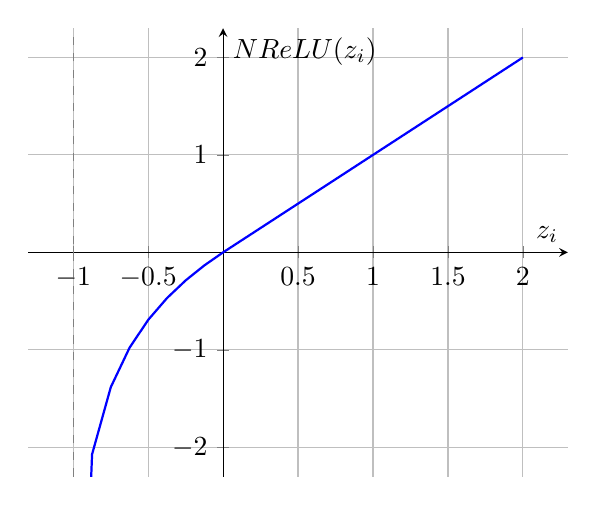
\begin{tikzpicture}
        \begin{axis}[
            xlabel={$z_i$},
            ylabel={$\text{NReLU}(z_i)$},
            xmin=-1.3, xmax=2.3,
            ymin=-2.3, ymax=2.3,
            axis lines=middle,
            grid=major,
            domain=-0.999:2, % Domínio para evitar o log de zero ou negativo
        ]
        % A função ln(1+x) está definida para x > -1
        \addplot[blue, thick] {x >= 0 ? x : ln(1+x)};
        % Linha vertical para mostrar a assíntota em z = -1
        \draw[dashed, gray] (axis cs:-1, -2.3) -- (axis cs:-1, 2.3);
        \end{axis}
    \end{tikzpicture}
    \label{fig:nrelu}
\end{figure}

Quando vamos calcular a sua derivada, encontramos um problema que não havia aparecido nas outras funções. O termo de ruído $\mathcal{N}$ é um termo não determísitico, o que significa que mesmo que tivéssemos a mesma entrada para a função Noisy ReLU duas ou mais vezes, não poderíamos afirmar com certeza de que essas saídas seriam iguais. Para resolver esses problemas, os autores consideram para a NReLU que sua função para o backward pass será irá retornar zero quando o valor de entrada for negativo ou nulo, e irá retornar um, quando o valor de entrada for positivo \parencite{Nair2010}. Então a expressão que representa a NReLU para a retroproagação é dada pela equação \ref{eq: DerivadaNReLU}, note que ela é a mesma expressão da derivada da ReLU tradicional.

\begin{equacaodestaque}{Derivada Noisy ReLU (NReLU)}
    \frac{d}{dz_i}[\text{NReLU}](z_i) = \begin{cases} 
    0 & \text{se } z_i \le 0 \\ 
    1 & \text{se } z_i > 0 
    \end{cases}
    \label{eq:nrelu-derivada}
\end{equacaodestaque}

Se a função da Noisy ReLU no backward pass será a mesma que a derivada da ReLU, podemos então utilizar como base o gráfico da derivada da ReLU. Para isso, temos então a figura \ref{fig:GraficoNReLUDerivada}.

\begin{figure}[htbp] % Use [htbp] para dar flexibilidade ao LaTeX
    \centering % Centraliza o gráfico na página
    \caption{Gráfico da função Backward Pass da Noisy ReLU}
    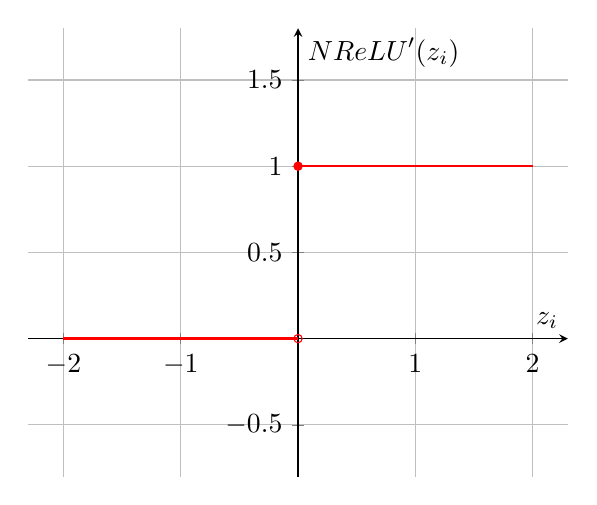
\begin{tikzpicture}
        \begin{axis}[
            xlabel={$z_i$},
            ylabel={$\text{NReLU}'(z_i)$},
            xmin=-2.3, xmax=2.3,
            ymin=-0.8, ymax=1.8,
            axis lines=middle,
            grid=major
        ]
        \addplot[red, thick, domain=-2:0] {0};
        \addplot[red, thick, domain=0:2] {1};
        \addplot[red, only marks, mark=o, mark size=1.5pt] coordinates {(0,0)};
        \addplot[red, only marks, mark=*, mark size=1.5pt] coordinates {(0,1)};
        \end{axis}
    \end{tikzpicture}
    \label{fig:nrelu-derivada}
\end{figure}

Ainda em \textit{Rectified Linear Units Improve Restricted Boltzmann Machines}, \textcite{Nair2010} citam que uma das propriedades interessantes da NReLU é a intensity equivarience (), a qual é bem útil para o reconhecimento de objetos. No texto, os autores destacam que um dos principais objetivos ao contruir um sistema que faça o reconhecimento de objetos, é garantir que a saída seja invariante às propriedades da sua entrada, como localização, escala, iluminação e orientação, e a NReLU é uma das fubções que quando adicionada em uma rede neural, garante que isso possa ser atingido \parencite{Nair2010}.

\textbf{Implementação em Python}

\section{O Problema dos Gradientes Explosivos}

Anteriormente, nós conhecemos as funções sigmoides, vimos que elas eram comumente utilizadas como as funções de ativação padrão de uma rede neural antes das funções retificadoras. Mas elas possuíam um problema, o do gradiente em fuga. Esse problema acontecia porque essas funções retornavam sempre números muito pequenos em suas derivadas, que consequentemente eram multiplicadas no \textit{backward pass} com o gradiente retropropagado gerando como produto um número pequeno, esse número era então novamente multiplicado por outra constante de baixo valor e por aí vai, como resultado, o gradiente retropropagado que chegava nas primeiras camadas para atualizar os pesos e vieses da rede possuía um valor tão pequeno que muitas vezes não resultava em uma atualização capaz de gerar impacto no aprendizado da rede. Assim, tínhamos o problema do gradiente em fuga.

Já nessa seção nós conhecemos a ReLU, e vimos que ela veio como uma alternativa para as funções sigmoides e que era capaz de corrigir esse problema. Contudo, ela também possui problemas, pelo fato de ser uma função que não é suturante como as sigmoides, isso faz com que ela possa gerar o problema da explosão do gradiente, para entendê-lo primeiro precisamos nos lembrar da fórmula do gradiente retropropagado.

\[
        \frac{\partial E}{\partial w_{ik}} = 
            \left( \sum_j \frac{\partial E}{\partial x_j} \cdot w_{ji} \right)
        \cdot 
            \sigma'(z_i)
        \cdot 
            a_k^{\text{ant}}
\]

O primeiro termo, o que possui o somatório, é responsável por calcular o erro total que chega para um neurônio $i$ da camada atual, para isso temos a equação \ref{eq: ErroRetropropagado}.

\begin{equation}
    \text{Erro}_i = \left( \sum_j \frac{\partial E}{\partial x_j} \cdot w_{ji} \right)
    \label{eq: ErroRetropropagado}
\end{equation}

$\partial E / \partial x_j$ nos indica o gradiente do erro em relação à saída de um neurônio $j$ que está na camada seguinte da rede. Para nós calcularmos ele, devemos aplicar a regra da cadeia, assim $\partial E / \partial x_j$ será dado pelo cálculo do erro vindo depois da camada $j$, uma camada $k$ por exemplo, assim, o erro será dado pela equação \ref{eq: ErroRetropropagadoK}.

\begin{equation}
    \text{Erro}_j = \left( \sum_k \frac{\partial E}{\partial x_k} \cdot w_{kj} \right)
    \label{eq: ErroRetropropagadoK}
\end{equation}

Note que temos um padrão nos cálculos dos erros.

\begin{enumerate}
    \item Para que nós possamos calcular o erro de uma camada $w_ba$ devemos encontrar o $\text{Erro}_b$;
    \item Para encontrar o $\text{Erro}_b$, precisamos calcular o gradiente da camada seguinte: $\partial E / \partial x_c$
    \item O gradiente ($\partial E / \partial x_c$) é calculado a partir do $\text{Erro}_c$
    \item Para calcular o $\text{Erro}_c$, precisamos da camada seguinte e seu gradiente $\partial E / \partial x_d$ que envolve os pesos $w_de$
    \item E assim por diante até a última camada da rede.
\end{enumerate}

Com base nessa análise podemos encontrar uma expressão que será capaz de nos mostrar qual será o valor do gradiente retropropagado agora considerando as atualizações de pesos que é feita na rede, ela é dada pela equação \ref{eq: GradienteRetropropagado}.

\begin{equation}
    \delta^l \propto (W^{l+1})^T \cdot (W^{l+2})^T \cdots (W^L)^T \cdot \delta^L 
    \label{eq: GradienteRetropropagado}
\end{equation} 

Note que, com base nessa expressão, se um cenário em que sempre houver valores muito grandes nos pesos das camadas da rede, ou ate mesmo muitas camadas, o gradiente que chegará na última camada poderá ter um valor muito alto, podendo atrapalhar o desempenho da rede neural e como ela irá aprender, assim temos um sério problema ao construir uma rede.

Esse tipo de problema, é chamado de problema da explosão do gradiente e ele pode ser definido da seguinte forma:

\begin{quote}
    Quando o erro é retropropagado por uma rede neural, ele pode aumentar exponencialmente de camada para camada. Nesses casos, o gradiente em relação aos parâmetros em camadas inferiores pode ser exponencialmente maior do que o gradiente em relação aos parâmetros em
    camadas superiores. Isso torna a rede difícil de treinar se ela for suficientemente profunda.
\end{quote}

\parencite[p.~2]{explodingGradient}

Assim, mesmo a ReLU corrigindo o problema do gradiente em fuga, ela acabou por introduzir uma nova categoria de problemas para uma rede neural. Acontecimentos assim são comuns, muitas vezes queremos concertar algo mas acabamos por atrapalhar outra parte de um projeto de rede neural, por isso, devemos escolher com calma quais funções serão utilizadas além de realizar testes para garantir uma melhor performance do modelo que está sendo criado.

\section{Comparativo de Desempenho das Funções Retificadoras}

Além do problema do explosão de gradientes que pode ocorrer ao utilizar a ReLU em uma rede neural, essa função também sofre de outro problema crônico: o do neurônios agonizantes (ou \textit{Dying ReLU Problem} em inglês). Esse problema pode ser definido como uma variação do problema do gradiente em fuga, em que uma parte dos neurônios da rede morrem e passam a retornar somente zero independente de sua entrada \parencite{dyingReLU}.

Para entendermos melhor devemos nos lembrar da estrutura básica de uma camada densa de neurônios de uma rede neural, de forma que ela pode ser vista na equação \ref{eq: EquacaoNeuronio2}, em que $W$ representa um vetor de pesos para os neurônios dessa camada, $X$ é o vetor de elementos de entrada e $b$ é o viés.

\begin{equation}
    y = W^T X + b
    \label{eq: EquacaoNeuronio2}
\end{equation}

Se estivemos utilizando a ReLU como função de ativação dessa camada, essa variável $y$ irá passar para uma função $\max(0, y)$, podem existir conjuntos de dados que quando passados por essa camada, a condição mais comum de ocorrer será a de $y < 0$ para os diferentes padrões de treinamento, isso tem efeito no \textit{backward pass}, em que vamos utilizar a derivada da ReLU, que também será zero para casos em que $y < 0$, e nós sabemos que com a derivada dessa função nós calculamos o gradiente que irá calcular o como o peso da rede irá mudar de uma época para outra, se essa saída for zero, quando ela for multiplicada ao calcular o gradiente ele também será zero, e consequentemente os pesos e vieses da rede neural não serão atualizados, se eles não são atualizados, o neurônio não aprende, tendo então o problema do neurônios agonizantes \parencite{douglasDyingRelu}.

Essa condição de vários neurônios morrendo causada pela ReLU acabou por gerar um novo conjunto de funções, as quais possuem propriedades comuns da ReLU, como a não linearidade e a simplicidade nos cálculos mas que buscam resolver ou amenizar esse problema em uma rede neural. Uma das funções que busca resolver esse problema é a Leaky ReLU \parencite{douglasDyingRelu}.

Agora que conhecemos a ReLU, vimos como ela surgiu e se popularizou, além de suas propriedades e problemas, podemos conhecer as suas variações, as quais buscam corrigir alguns problemas que a função original possui mas mesmo assim mantendo as sua essência como inspiração para a criação de uma função melhor. Primeiro, conheceremos as variações com vazamentos, começando pela Leaky ReLU ou LReLU.